\chapter{Language-Specific Neurons and Cross-Lingual Transfer}
\label{ch:neurons}

\section{Introduction}
\label{sec:neurons-intro}

\subsection{Motivation}
\label{subsec:neurons-motivation}

Multilingual models handle many languages with a single set of parameters, and one
open question is whether the information a model uses for a given language sits in
an identifiable part of the network. Work on language-specific neurons proposes
that it does. The claim is that a small number of neurons in the feed-forward
layers activate mainly for one language and stay quiet for others, and that these
neurons can be located from activation statistics
\citep{tang2024language, kojima2024multilingual}.

If this holds in a strong form, it points to a direct way to help low-resource
languages, where models tend to do worse than on high-resource ones. The idea would
be to find the neurons for a target language and change them, either at test time
or through fine-tuning, so that the model handles that language better. This is the
possibility we examine in this chapter.

Earlier work has shown that these neurons can control which language a model
generates text in. Turning them on or off pushes the model to produce output in a
given language or moves it away from that language
\citep{tang2024language, kojima2024multilingual}. This is a result about the
\emph{form} of the output, that is, the language the model writes in. It does not
say whether the neurons matter for the \emph{content} of a task, such as deciding
whether one sentence entails another or finding the answer to a question. Those
tasks need the model to use what it knows, not only to write in a particular
language. Whether language-specific neurons help on such tasks for low-resource
languages is the question we study here.

\subsection{Problem Statement}
\label{subsec:neurons-problem}

We study whether interventions on language-specific neurons improve cross-lingual
performance on downstream tasks. By cross-lingual transfer we mean the following
setting: the model is adapted using a source language, here English, for which
labelled data is available, and is then evaluated on a target language for which
we do not use task training data. If language-specific neurons carry the
information that lets the model handle a target language, then acting on those
neurons should raise target-language performance.

We make this concrete in two ways. First, we change the activations of the
identified neurons at test time, replacing them with statistical values computed
from a multilingual corpus, and measure the effect on the task. Second, we
fine-tune only the identified neurons with a low-rank adapter, so that the update
is restricted to those neurons, and again measure the effect. We run both kinds of
intervention on two tasks, natural language inference with XNLI
\citep{conneau2018xnli} and extractive question answering with XQuAD
\citep{artetxe2020cross}, using two models, Llama~3.1 \citep{grattafiori2024llama}
and Mistral Nemo \citep{mistral2024nemo}. We also compare two ways of identifying
the neurons, so that the conclusion does not depend on a single method.

\subsection{Contributions}
\label{subsec:neurons-contributions}

This chapter, based on our published work \citep{mondal2025language}, reports the
following.

\begin{itemize}
	\item We test two neuron identification methods, Language Activation
	Probability Entropy and activation-probability thresholding, on Llama~3.1 and
	Mistral Nemo, and two intervention types, test-time activation edits and
	neuron-targeted low-rank fine-tuning, on XNLI and XQuAD.
	
	\item We find that these interventions do not give consistent improvements on
	cross-lingual downstream tasks for low-resource languages. Where there is any
	gain it is small and not in a consistent direction, and several interventions
	degrade performance, sometimes sharply, more so for Mistral Nemo and on XQuAD.
	
	\item We report two further observations that explain the negative result.
	Setting a neuron's activation to zero does not remove its effect, which means
	zero is not a reliable way to turn a neuron off. And the neurons identified for
	different languages are not independent, so editing the neurons for one
	language affects others. These are consistent with neurons that take part in
	more than one function \citep{elhage2022superposition}.
\end{itemize}

The negative result here is the reason the rest of the thesis moves away from
editing internal components and towards methods that act on the training
objective.

\section{Background and Preliminaries}
\label{sec:neurons-background}

\subsection{Definition of a Neuron}
\label{subsec:neurons-definition}

We work with neurons in the feed-forward, or MLP, block of a transformer layer.
This subsection fixes what a neuron is so that the identification and intervention
methods later are precise.

Consider layer $i$ of a transformer. Let $H_{i-1} \in \mathbb{R}^{T \times d}$ be
the hidden states from the previous layer, where $T$ is the sequence length and
$d$ is the model dimension. The layer first applies multi-head self-attention. We
write its output as
\begin{equation}
	\hat{H}_i = \mathrm{Attn}\!\left(H_{i-1} W^i_q,\; H_{i-1} W^i_k,\; H_{i-1} W^i_v\right) W^i_o,
	\label{eq:neurons-attn}
\end{equation}
where $W^i_q, W^i_k, W^i_v, W^i_o \in \mathbb{R}^{d \times d}$ are the projection
matrices of the attention module and $\mathrm{Attn}(\cdot)$ is scaled dot-product
attention. The MLP block takes $\hat{H}_i$ as input.

In a standard transformer MLP, the block applies an up-projection, a non-linear
activation, and a down-projection:
\begin{equation}
	h_i = \mathrm{act\_fn}\!\left(\hat{H}_i W^i_1\right) W^i_2,
	\label{eq:neurons-mlp}
\end{equation}
where $W^i_1 \in \mathbb{R}^{d \times 4d}$ and $W^i_2 \in \mathbb{R}^{4d \times d}$
are the up- and down-projection matrices, and $\mathrm{act\_fn}(\cdot)$ is a
non-linear activation such as GELU or SiLU. The intermediate width is commonly
$4d$, though the exact factor depends on the model.

We define a neuron as one coordinate of the intermediate activation. The $j$-th
neuron of layer $i$ is
\begin{equation}
	h_{i,j} = \mathrm{act\_fn}\!\left(\left(\hat{H}_i W^i_1\right)_j\right),
	\label{eq:neurons-neuron}
\end{equation}
where $\left(\hat{H}_i W^i_1\right)_j$ is the pre-activation value of that neuron.
A neuron in this sense is a single hidden unit in the MLP, and its activation is a
scalar for each input token.

% FIGURE 3.1 -- include here.
% Suggested filename: fig_mlp_glu_architecture.pdf
% Content: schematic of the MLP/GLU block in a Llama-style layer, showing the
% self-attention output feeding the gate projection (W1), up projection (W3),
% the elementwise product after the SiLU activation, and the down projection (W2).
% Mark the j-th neuron on the intermediate (4d-wide) activation.
\begin{figure}[t]
	\centering
	 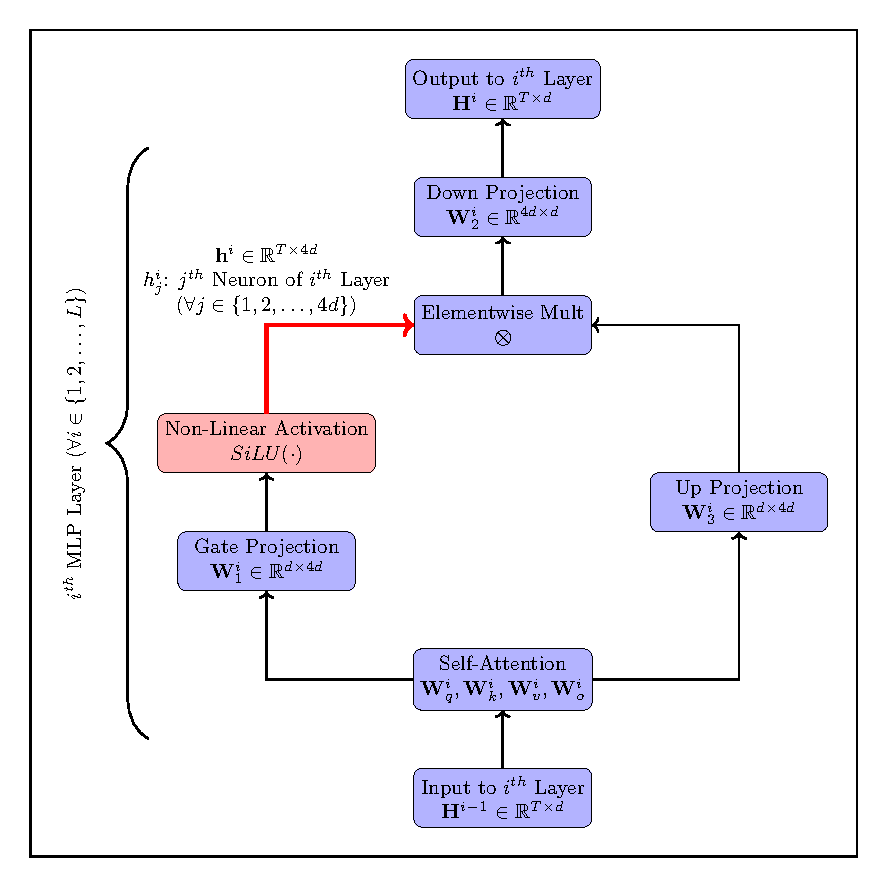
\includegraphics[width=0.8\linewidth]{Chapters/Chapter_3/mlp.pdf}
	\caption{Architecture of the MLP block in a Llama-style model. The output of
		self-attention is passed through a gate projection and an up projection, combined
		by an elementwise product after a SiLU activation, and then passed through a down
		projection. A neuron is one coordinate of the intermediate activation.}
	\label{fig:neurons-mlp-architecture}
\end{figure}

Recent models such as Llama use a gated variant of the MLP, the Gated Linear Unit
\citep{shazeer2020glu}. Here an extra projection $W^i_3$ gates the activation:
\begin{equation}
	h_i = \left[\mathrm{act\_fn}\!\left(\hat{H}_i W^i_1\right) \otimes \left(\hat{H}_i W^i_3\right)\right] W^i_2,
	\label{eq:neurons-glu}
\end{equation}
where $W^i_3 \in \mathbb{R}^{d \times 4d}$ and $\otimes$ is the elementwise
product. The gating lets the block represent richer transformations than the plain
MLP. The definition of a neuron does not change: it is still one coordinate of the
intermediate activation, now formed by the gated product.
Figure~\ref{fig:neurons-mlp-architecture} shows the block. Both models in this
chapter, Llama~3.1 and Mistral Nemo, use this gated form, so all neuron statistics
and interventions below act on the intermediate activations of
Equation~\ref{eq:neurons-glu}.

\subsection{Notation and Problem Setup}
\label{subsec:neurons-notation}

We collect the notation used in the rest of the chapter. A neuron is indexed by
its layer $i$ and position $j$ within that layer, written $(i,j)$. For an input
token at position $t$ in a sequence $s$, the activation of neuron $(i,j)$ is a
scalar, which we write $h^{(s,t)}_{i,j}$. We compute statistics of these
activations over a corpus, separately for each language, to decide which neurons
are specific to a language. The details of these statistics are in
Section~\ref{subsec:neurons-statistics}.

We consider a set of languages $L$. For a language $l \in L$, the identification
methods return a set of neurons $N_l$ that the method marks as specific to $l$. An
intervention is a change applied to the neurons in $N_l$, either replacing their
activations at test time or restricting fine-tuning to them. We evaluate the
effect of an intervention on a downstream task in a target language.

For the downstream tasks, we use a source language, English, for adaptation and a
target language for evaluation, and we do not use task training data in the target
language. This is the cross-lingual transfer setting described in
Section~\ref{subsec:neurons-problem}. The two tasks, XNLI and XQuAD, and their
evaluation metrics are defined in Section~\ref{sec:neurons-setup}.

\section{Identifying Language-Specific Neurons}
\label{sec:neurons-identify}

This section describes how we find the neurons that a method marks as specific to
a language. We first describe the corpus and the activation statistics we compute
from it (Section~\ref{subsec:neurons-statistics}), then the two identification
methods we use, Language Activation Probability Entropy
(Section~\ref{subsec:neurons-lape}) and activation-probability thresholding
(Section~\ref{subsec:neurons-actprob}), and finally the language sets we run them
on (Section~\ref{subsec:neurons-langsets}).

\subsection{Activation Statistics from a Multilingual Corpus}
\label{subsec:neurons-statistics}

To find language-specific neurons we first need a record of how each neuron
behaves on each language. We collect this from a multilingual corpus drawn from
Wikipedia \citep{wikidump}, using a subset of languages. Each language's text is
tokenized and passed through the model, and we record the activations from the MLP
modules.

Let $h^{t}_{i,j}$ be the activation of neuron $(i,j)$ at token position $t$ in a
sequence of length $T$. For a single sequence, the mean activation of the neuron
over its tokens is
\begin{equation}
	\bar{h}_{i,j} = \frac{1}{T} \sum_{t=1}^{T} h^{t}_{i,j}.
	\label{eq:neurons-seqmean}
\end{equation}
For a language $l$ with a set of sequences $\mathcal{S}_l$, we average over all
sequences to get a per-language profile of the neuron,
\begin{equation}
	h^{l}_{i,j} = \frac{1}{|\mathcal{S}_l|} \sum_{s \in \mathcal{S}_l} \bar{h}^{(s)}_{i,j}.
	\label{eq:neurons-langmean}
\end{equation}

Besides the mean, we compute the standard deviation and a set of quantiles of the
activations for each neuron and language, since some identification methods use
them. The $q$-quantile of a neuron's activation is
\begin{equation}
	P_q(h_{i,j}) = \inf\left\{ x \in \mathbb{R} : F_{h_{i,j}}(x) \geq q \right\},
	\label{eq:neurons-quantile}
\end{equation}
where $F_{h_{i,j}}$ is the cumulative distribution function of the neuron's
activations. We compute the 5th, 10th, 25th, 50th, 75th, 90th, and 95th
percentiles. These statistics, computed once per language, are the input to the
identification methods below and also to the test-time interventions in
Section~\ref{sec:neurons-intervene}.

\subsection{Language Activation Probability Entropy (LAPE)}
\label{subsec:neurons-lape}

The first method is Language Activation Probability Entropy (LAPE)
\citep{tang2024language}. The idea is that a neuron is specific to a language if it
tends to activate for that language and not for others. LAPE measures this with the
entropy of a neuron's activation probabilities across languages: a low entropy
means the neuron activates for one or a few languages, while a high entropy means
it activates evenly across all of them.

\paragraph{Step 1: Activation probabilities.}
For a language $l$, the activation probability of neuron $(i,j)$ is the fraction of
tokens for which the neuron has a positive activation,
\begin{equation}
	p^{l}_{i,j} = \mathbb{E}\left[ \mathbb{I}\!\left( h^{l}_{i,j} > 0 \right) \right],
	\label{eq:neurons-lape-prob}
\end{equation}
where $\mathbb{I}(\cdot)$ is the indicator function and the expectation is over all
tokens in all sequences for language $l$.

\paragraph{Step 2: Normalize across languages.}
For a set of $k$ languages, we normalize the probabilities so that they form a
distribution over languages for each neuron,
\begin{equation}
	\mathcal{P}^{l}_{i,j} = \frac{p^{l}_{i,j}}{\sum_{l'=1}^{k} p^{l'}_{i,j}}.
	\label{eq:neurons-lape-norm}
\end{equation}

\paragraph{Step 3: Entropy.}
The LAPE value of a neuron is the entropy of this distribution,
\begin{equation}
	\mathrm{LAPE}(i,j) = - \sum_{l=1}^{k} \mathcal{P}^{l}_{i,j} \log \mathcal{P}^{l}_{i,j}.
	\label{eq:neurons-lape-entropy}
\end{equation}
A small LAPE value marks a neuron that activates for few languages.
Figure~\ref{fig:neurons-lape-procedure} shows the steps.

% FIGURE 3.2 -- include here.
% Suggested filename: fig_lape_procedure.pdf
% Content: bottom-to-top flow for one neuron: per-language neuron activations ->
% unnormalized activation probabilities p^l_{i,j} -> normalized probabilities
% P^l_{i,j} -> LAPE entropy value. (This is the BPS1 LAPE figure.)
\begin{figure}[ht]
	\centering
	 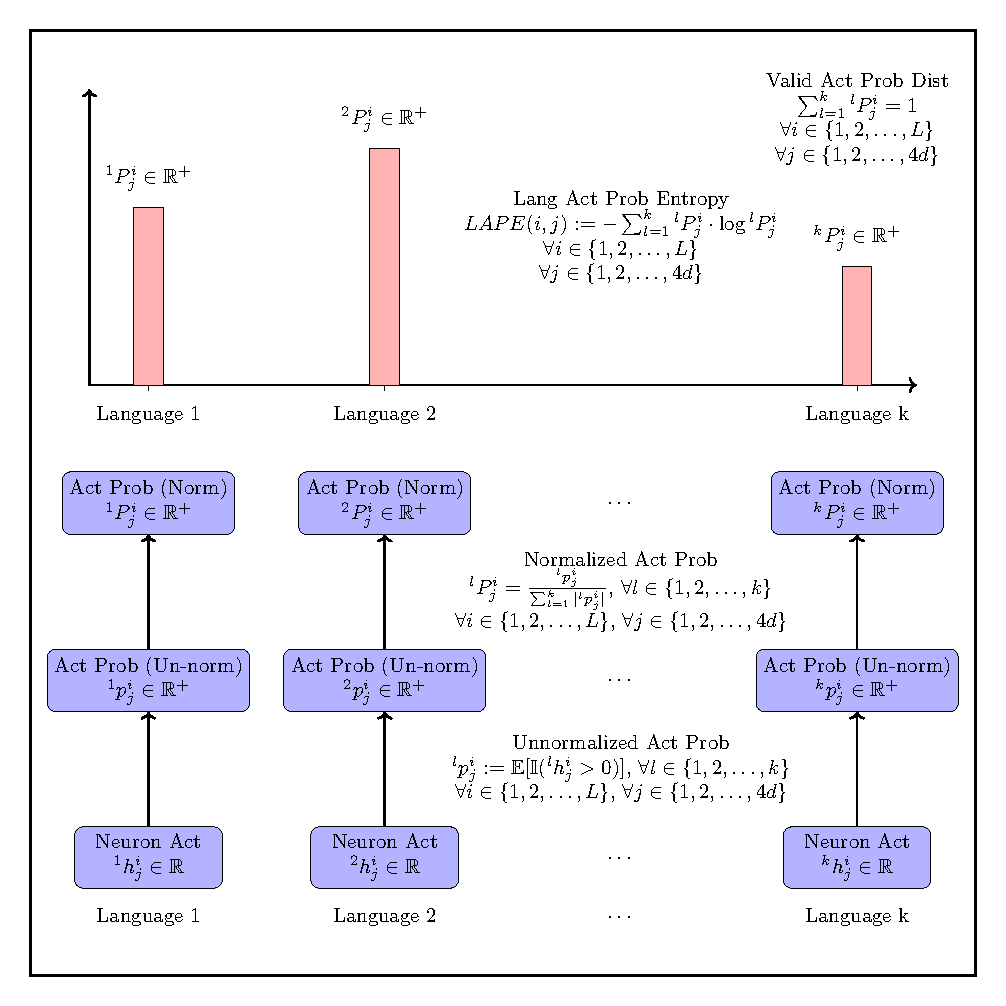
\includegraphics[width=0.8\linewidth]{Chapters/Chapter_3/lape.pdf}
	\caption{Computing LAPE for a single neuron. For each language we measure the
		probability that the neuron activates, normalize these probabilities across
		languages into a distribution, and take its entropy. Neurons with low entropy
		activate for only a few languages.}
	\label{fig:neurons-lape-procedure}
\end{figure}

\paragraph{Step 4: Threshold and selection.}
A neuron is only considered if it activates often enough for at least one language.
We set a threshold at the 95th percentile of the activation probabilities over all
neurons and languages,
\begin{equation}
	\mathrm{Threshold} = \mathrm{Quantile}_{0.95}\!\left( p_{i,j} \mid \forall i,j,l \right),
	\label{eq:neurons-lape-threshold}
\end{equation}
and keep neuron $(i,j)$ only if $p^{l}_{i,j} > \mathrm{Threshold}$ for some
language $l$. Among the neurons that pass, we select the ones with the lowest LAPE
values. We take the bottom $1\%$ of all neurons,
\begin{equation}
	m = \frac{1}{100} \times 4d \times L,
	\label{eq:neurons-lape-m}
\end{equation}
where $L$ is the number of layers and $4d$ the number of neurons per layer. Each
selected neuron is then assigned to the languages for which it activates above the
threshold, which gives the per-language neuron sets $N_l$.

\subsection{Activation-Probability Thresholding (Act Prob 90p)}
\label{subsec:neurons-actprob}

The second method scores each neuron by how often it activates strongly for a
language, and keeps the top-scoring neurons per language. We use this as a check
against LAPE, so that the conclusion does not rest on one identification method.
We refer to it as Act Prob 90p, after the relevance score we use.

\paragraph{Relevance score.}
For each neuron and language we compute a relevance value $r^{l}_{i,j}$. Several
choices are possible. The simplest is the activation probability, the fraction of
tokens with a positive activation,
\begin{equation}
	r^{l}_{i,j} = \mathbb{E}\left[ \mathbb{I}\!\left( h^{l}_{i,j} > 0 \right) \right].
	\label{eq:neurons-act-zero}
\end{equation}
We can also use the mean absolute activation, the probability of exceeding the
layer mean, or the probability of exceeding the 90th-percentile activation. The
last of these is the score we use in the main experiments,
\begin{equation}
	r^{l}_{i,j} = \mathbb{E}\left[ \mathbb{I}\!\left( h^{l}_{i,j} > P90^{l}_{i,j} \right) \right],
	\label{eq:neurons-act-90p}
\end{equation}
where $P90^{l}_{i,j}$ is the 90th percentile of the neuron's activations for
language $l$. This score picks out neurons that have rare but strong activations,
which we take as a sign of a specialized response.

\paragraph{Selection.}
For each language $l$ we collect the relevance values into a tensor
$R^{l} = \{ r^{l}_{i,j} \}$ and keep the top $m$ neurons by relevance. Here we use
\begin{equation}
	m = \frac{0.125}{100} \times L \times 4d,
	\label{eq:neurons-act-m}
\end{equation}
and the per-language set is
\begin{equation}
	N_l = \left\{ (i,j) \mid (i,j) \in \mathrm{Top}_m(R^{l}) \right\}.
	\label{eq:neurons-act-set}
\end{equation}
LAPE and Act Prob 90p differ in how they score and select neurons, so if both lead
to the same conclusion about interventions, the result is less likely to be an
artifact of one method.

\subsection{Language Sets}
\label{subsec:neurons-langsets}

We run the identification on two groups of languages, which we call Set1 and Set6.
Set1 is a mixed group covering several scripts and language families, used to study
neurons across languages that the model handles with varying success. Set6 is a
group of Indian languages, used to look more closely at the low-resource case that
is the focus of this chapter. Set1 covers English, French, Spanish, Vietnamese, Indonesian, Japanese, and Chinese, a mixed group across several scripts and families. Set6 covers English, Bengali, Hindi, Tamil, Telugu, Marathi, Urdu, Kannada, Malayalam, and Punjabi, the group of Indian
languages used to look more closely at the low-resource case. English is included
in both sets as the source language. We compute the activation statistics and run
both identification methods separately for each set, since the set of languages
changes the normalization in LAPE (Equation~\ref{eq:neurons-lape-norm}) and
therefore which neurons are selected.

\section{Intervening on Language-Specific Neurons}
\label{sec:neurons-intervene}

Having identified the neurons, we now change them and measure the effect. We use
two kinds of intervention. The first replaces neuron activations at test time
(Section~\ref{subsec:neurons-testtime}). The second fine-tunes only the identified
neurons (Section~\ref{subsec:neurons-lora}). We also describe a perplexity-based
probe (Section~\ref{subsec:neurons-ppxc}) that we use to check whether a test-time
intervention is doing anything to the model's handling of a language.

\subsection{Test-Time Interventions}
\label{subsec:neurons-testtime}

In a test-time intervention we run the model as usual, but for the neurons in
$N_l$ we replace the activation that the model would have produced with a fixed
value taken from the statistics in Section~\ref{subsec:neurons-statistics}. The
value is the same for every token, and the rest of the model runs unchanged. This
lets us ask whether forcing the language-specific neurons to a particular level
changes the model's behaviour on the target language.

We try several replacement values. The mean activation $\mu$ for the language sets
the neuron to its typical level. The higher percentiles, $P75$, $P90$, and $P95$,
push the neuron towards strong activation. The lower percentiles, $P25$, $P10$, and
$P5$, push it towards weak activation. We also try setting the activation to zero,
which is often described as turning the neuron off. As we show later
(Section~\ref{sec:neurons-results-transfer}), setting the activation to zero is not
the same as removing the neuron's effect, because zero is not a neutral value for
these activations.

\subsection{Perplexity Change as a Probe}
\label{subsec:neurons-ppxc}

Before measuring downstream task accuracy, it helps to check whether an
intervention affects the model's basic handling of a language at all. We use
perplexity for this. If the neurons in $N_l$ matter for language $l$, then
intervening on them should change the model's perplexity on text in language $l$.

We define the perplexity change $\mathrm{PPXC}(i,j)$ as the difference between the
perplexity on language $j$ after intervening on the neurons identified for language
$i$ and the perplexity with no intervention,
\begin{equation}
	\mathrm{PPXC}(i,j) = \mathrm{PPX}\!\left( j \mid \text{intervention on } i \right) - \mathrm{PPX}(j).
	\label{eq:neurons-ppxc}
\end{equation}
A value near zero means the intervention barely touches the model's handling of
language $j$. A large value means the intervention has a strong effect. Comparing
the diagonal entries ($i = j$, intervening on a language's own neurons) with the
off-diagonal entries ($i \neq j$, intervening with another language's neurons)
shows how specific the neurons are to their own language.

\subsection{Neuron-Targeted Fine-Tuning with LoRA}
\label{subsec:neurons-lora}

The second intervention fine-tunes the identified neurons rather than fixing their
activations. We use Low-Rank Adaptation (LoRA) \citep{hu2022lora}, which adds a
low-rank update $\Delta W$ to a weight matrix while leaving the pretrained weight
$W$ unchanged. The update is factored as
\begin{equation}
	\Delta W = A \cdot B,
	\label{eq:neurons-lora}
\end{equation}
with $A \in \mathbb{R}^{d_\text{in} \times r}$ and
$B \in \mathbb{R}^{r \times d_\text{out}}$, where the rank $r$ is much smaller than
$d_\text{in}$ or $d_\text{out}$.

To restrict the update to the identified neurons, we apply a binary mask to the
factors,
\begin{equation}
	A = \mathrm{mask}_A \cdot A_t, \qquad B = \mathrm{mask}_B \cdot B_t,
	\label{eq:neurons-lora-mask}
\end{equation}
where $A_t$ and $B_t$ are the trainable matrices. We leave $\mathrm{mask}_A$ all
ones, and in $\mathrm{mask}_B$ we set to zero the columns that correspond to
neurons we want to freeze. For a frozen neuron index $j_f$,
\begin{equation}
	[\mathrm{mask}_B]_{i,j} =
	\begin{cases}
		0, & \text{if } j = j_f, \; j_f \in \text{Frozen Neurons}, \\
		1, & \text{otherwise.}
	\end{cases}
	\label{eq:neurons-lora-maskb}
\end{equation}
This makes $\Delta W_{i,j} = 0$ for every frozen neuron, so no update reaches it.
The fine-tuned MLP output is then
\begin{equation}
	y = x \cdot W + x \cdot \Delta W,
	\label{eq:neurons-lora-out}
\end{equation}
where only the selected neurons receive an update through $\Delta W$.
Figure~\ref{fig:neurons-lora} illustrates the masking for a small example.

% FIGURE 3.3 -- include here.
% Suggested filename: fig_masked_lora.pdf
% Content: the BPS1 masked-LoRA diagram. Show DeltaW = A.B, the mask zeroing the
% columns of B for frozen neurons (e.g. neurons 3 and 5 frozen, LoRA rank 2),
% and the resulting DeltaW with zero columns at the frozen positions.
\begin{figure}[ht]
	\centering
	 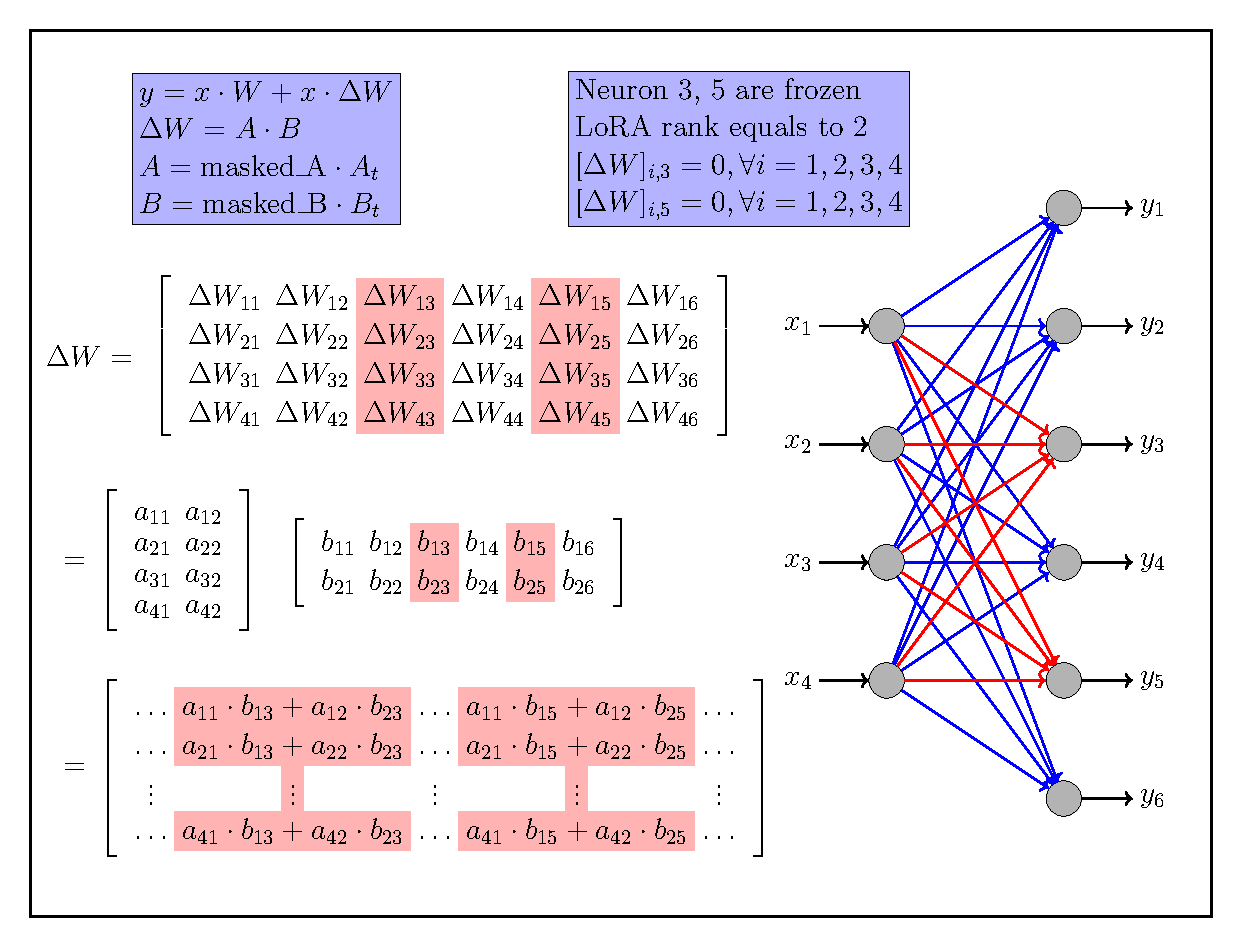
\includegraphics[width=0.8\linewidth]{Chapters/Chapter_3/lora.pdf}
	\caption{Neuron-targeted fine-tuning with masked LoRA. The low-rank update
		$\Delta W = A \cdot B$ is masked so that the columns of $B$ for frozen neurons
		are set to zero. In the example, neurons 3 and 5 are frozen with LoRA rank 2,
		so the corresponding columns of $\Delta W$ are zero and only the remaining
		neurons are updated.}
	\label{fig:neurons-lora}
\end{figure}

Alongside the masked MLP update, we always fine-tune the attention projections
($q$, $k$, $v$, $o$) and the task-specific head with ordinary LoRA. This keeps the
task performance reasonable, so that the comparison is between updating the
identified neurons and not updating them, rather than between training and not
training at all.

\subsection{Fine-Tuning Configurations}
\label{subsec:neurons-config}

We vary which language's neurons are fine-tuned. We refer to this as the
fine-tuning language (FTL). In one setting we fine-tune the neurons identified for
the source language, English. In another we fine-tune the neurons for the target
language. In a third we fine-tune the union of both. In all cases the task training
data is English, since we are testing cross-lingual transfer and do not use
target-language task data. Comparing these settings shows whether it matters which
language's neurons are made trainable, which is a direct test of whether the
language-specific sets carry transferable information.

\section{Experimental Setup}
\label{sec:neurons-setup}

\subsection{Models}
\label{subsec:neurons-models}

We use two pretrained multilingual models. Llama~3.1 \citep{grattafiori2024llama}
is an 8-billion-parameter model from Meta. Mistral Nemo \citep{mistral2024nemo} is
a 12-billion-parameter model. Both use the gated MLP of
Equation~\ref{eq:neurons-glu}, so the neuron definition and the identification
methods apply to both without change. We load both models in 4-bit precision to
reduce memory use.

\subsection{Tasks and Datasets}
\label{subsec:neurons-tasks}

\paragraph{XNLI.}
The Cross-lingual Natural Language Inference (XNLI) benchmark
\citep{conneau2018xnli} tests whether a model can decide the relationship between
two sentences across languages. Given a premise and a hypothesis, the model labels
the pair as entailment, neutral, or contradiction. We use English as the source
language and evaluate on lower-resource target languages from our language sets. We
form the input by joining the premise and hypothesis with a separator token and
tokenize to a maximum length of 512 tokens.

\paragraph{XQuAD.}
The Cross-lingual Question Answering Dataset (XQuAD) \citep{artetxe2020cross} tests
extractive question answering across languages. Given a passage and a question, the
model must select the span of the passage that answers the question. As with XNLI,
we adapt using English and evaluate on the target languages, without using
target-language task data.

\subsection{Implementation Details}
\label{subsec:neurons-impl}

For neuron identification we collect activations on the Wikipedia corpus
\citep{wikidump} with a maximum sequence length of 512 tokens. For fine-tuning we
use LoRA on the MLP neurons as described in
Section~\ref{subsec:neurons-lora}, together with LoRA on the attention projections
and the task head. We train with the AdamW optimizer and mixed-precision
computation. The full list of hyperparameters, including LoRA rank, scaling factor,
learning rate, number of epochs, and batch size for each task, is given in
Table~\ref{tab:neurons-hyperparams}.

\subsection{Evaluation Metrics}
\label{subsec:neurons-metrics}

For XNLI we report classification accuracy on the three-way label. For XQuAD we
report exact match and F1 between the predicted span and the reference answer. For
the neuron analysis we report the perplexity change $\mathrm{PPXC}$ of
Equation~\ref{eq:neurons-ppxc}, along with counts and overlaps of the identified
neurons. The no-intervention numbers in
Section~\ref{sec:neurons-results-transfer} serve as the baseline against which all
interventions are compared.

\section{Results: Neuron Analysis}
\label{sec:neurons-results-analysis}

Before looking at task performance, we study the neurons that the two methods
identify. This tells us how many neurons are marked per language, how much the
sets overlap across languages, where they sit in the model, and whether
intervening on them changes the model's handling of a language at all. We run this
analysis on the two language sets, Set1 and Set6, described in
Section~\ref{subsec:neurons-langsets}.

\subsection{Number of Language-Specific Neurons}
\label{subsec:neurons-counts}

Figure~\ref{fig:neurons-counts} shows the number of neurons identified per language
by LAPE, for both models on Set1 and Set6. The counts vary by language and are a
small fraction of the total number of neurons, as expected from the selection rule
in Equation~\ref{eq:neurons-lape-m}. The Act Prob 90p method works differently: by
construction it keeps a fixed number of top-scoring neurons per language
(Equation~\ref{eq:neurons-act-m}), which is $573$ per language for Llama~3.1 and
$717$ for Mistral Nemo, so its per-language counts are equal and we do not plot
them. Either way the identified set is small. This sets up the rest of the analysis:
the neurons are few enough that, if they carried language-specific function in a
clean way, intervening on them should be both possible and visible.

% FIGURE 3.4 -- include here.
% Suggested filename: fig_neuron_counts.pdf
% Content: bar charts of the number of language-specific neurons per language,
% LAPE vs Act Prob 90p, for Llama 3.1 and Mistral Nemo, on Set1 and Set6.
\begin{figure}[ht]
	\centering
	 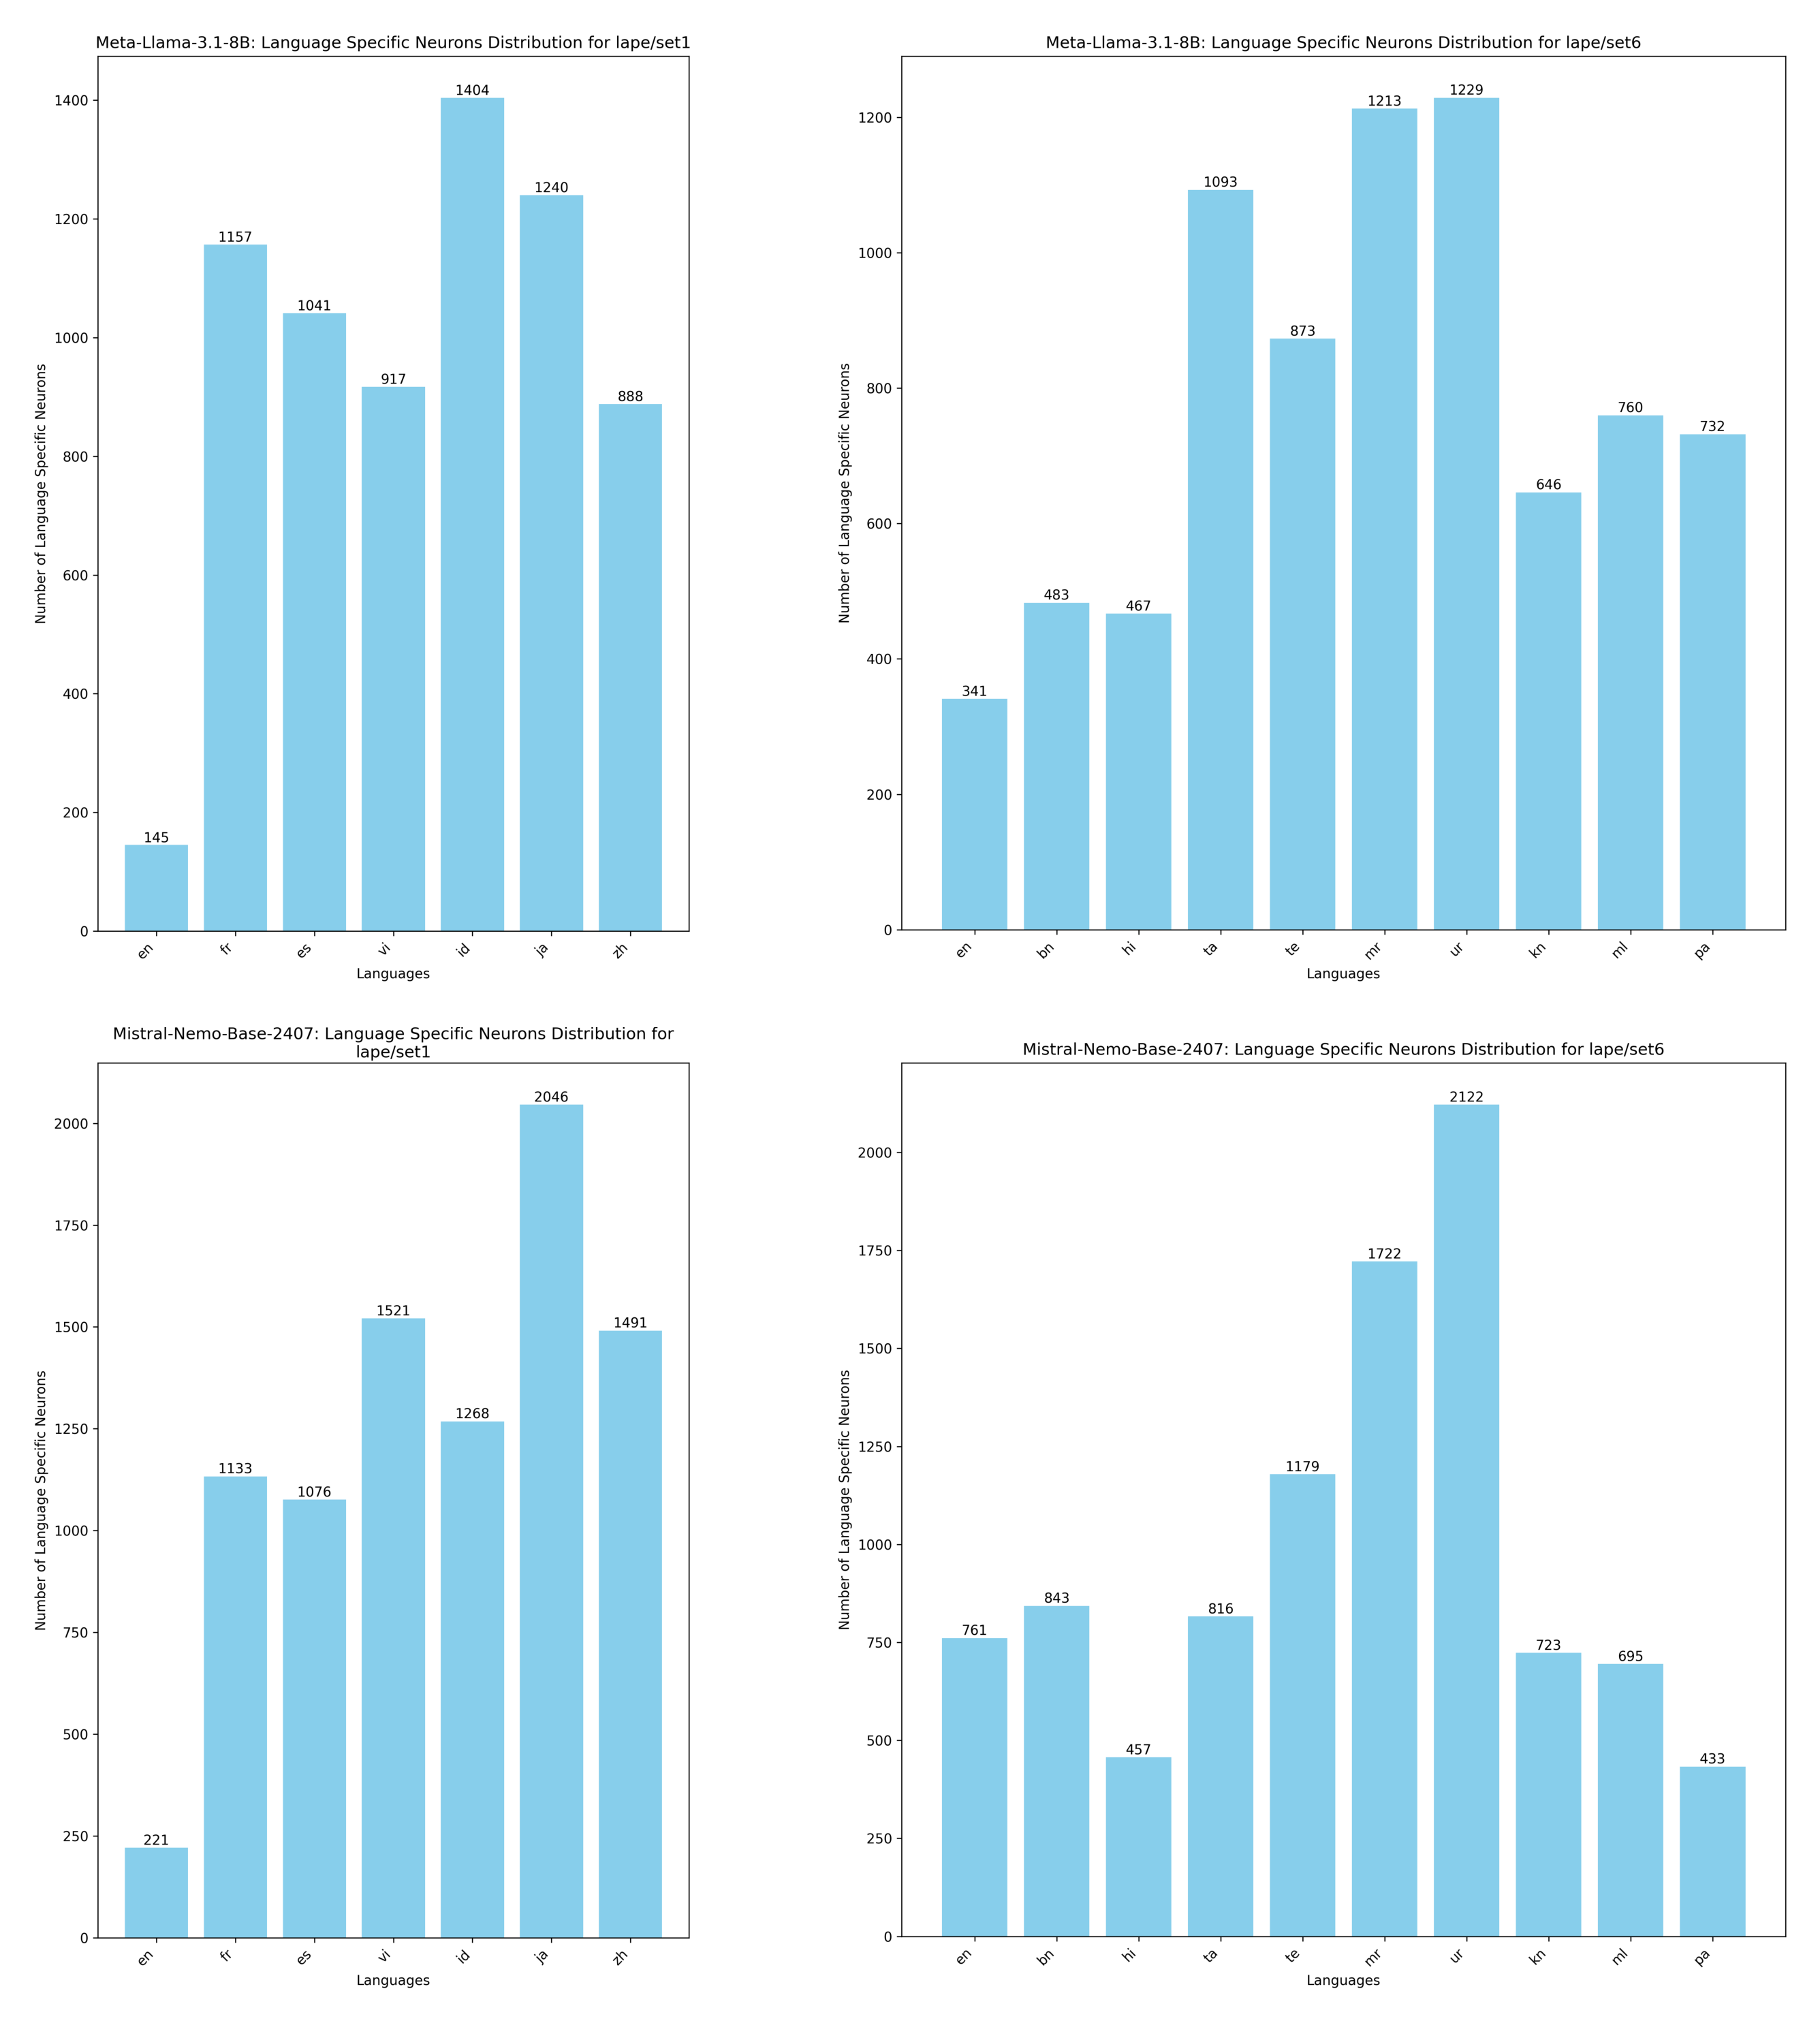
\includegraphics[width=0.8\linewidth]{Chapters/Chapter_3/figures/results/combined_lang_neuron_dist.png}
	\caption{Number of language-specific neurons identified per language by LAPE  for Llama~3.1 and Mistral Nemo on Set1 and Set6. Both models
		assign a small set of neurons to each language.}
	\label{fig:neurons-counts}
\end{figure}

\subsection{Overlap Between Languages}
\label{subsec:neurons-overlap}

If a neuron were specific to one language, it would appear in the set for that
language and no other. To check this, we count how many neurons are shared between
each pair of languages. Figure~\ref{fig:neurons-overlap-actprob} shows the overlap
for Act Prob 90p, and Figure~\ref{fig:neurons-overlap-lape} shows it for LAPE. In
each heatmap the diagonal is the size of a language's own set, and an off-diagonal
entry is the number of neurons two languages have in common.

The sets are far from disjoint. Under Act Prob 90p, where each language has 573
neurons in Llama~3.1 and 717 in Mistral Nemo, the shared counts between pairs of
languages often run to a few hundred, so a sizable part of any one set is not
unique to that language. LAPE shows the same thing on its larger sets. The amount
of sharing also tracks how close the languages are: pairs such as Japanese and
Chinese in Set1 overlap much more than unrelated pairs, and the Indian languages in
Set6 overlap most among themselves.

This is the first sign that the identified neurons are not cleanly tied to a single
language, and it matters for the interventions that follow. If a neuron belongs to
several languages at once, it cannot be changed for one of them without affecting
the others, so there is no clean way to act on a single target language through
these sets.

% FIGURE 3.5a (Act Prob 90p) -- include here.
% Suggested filename: fig_neuron_overlap_actprob.png
% Content: pairwise neuron-set overlap heatmaps for Act Prob 90p, for Llama 3.1 and
% Mistral Nemo (en, vi, ur, hi, zh).
\begin{figure}[ht]
	\centering
	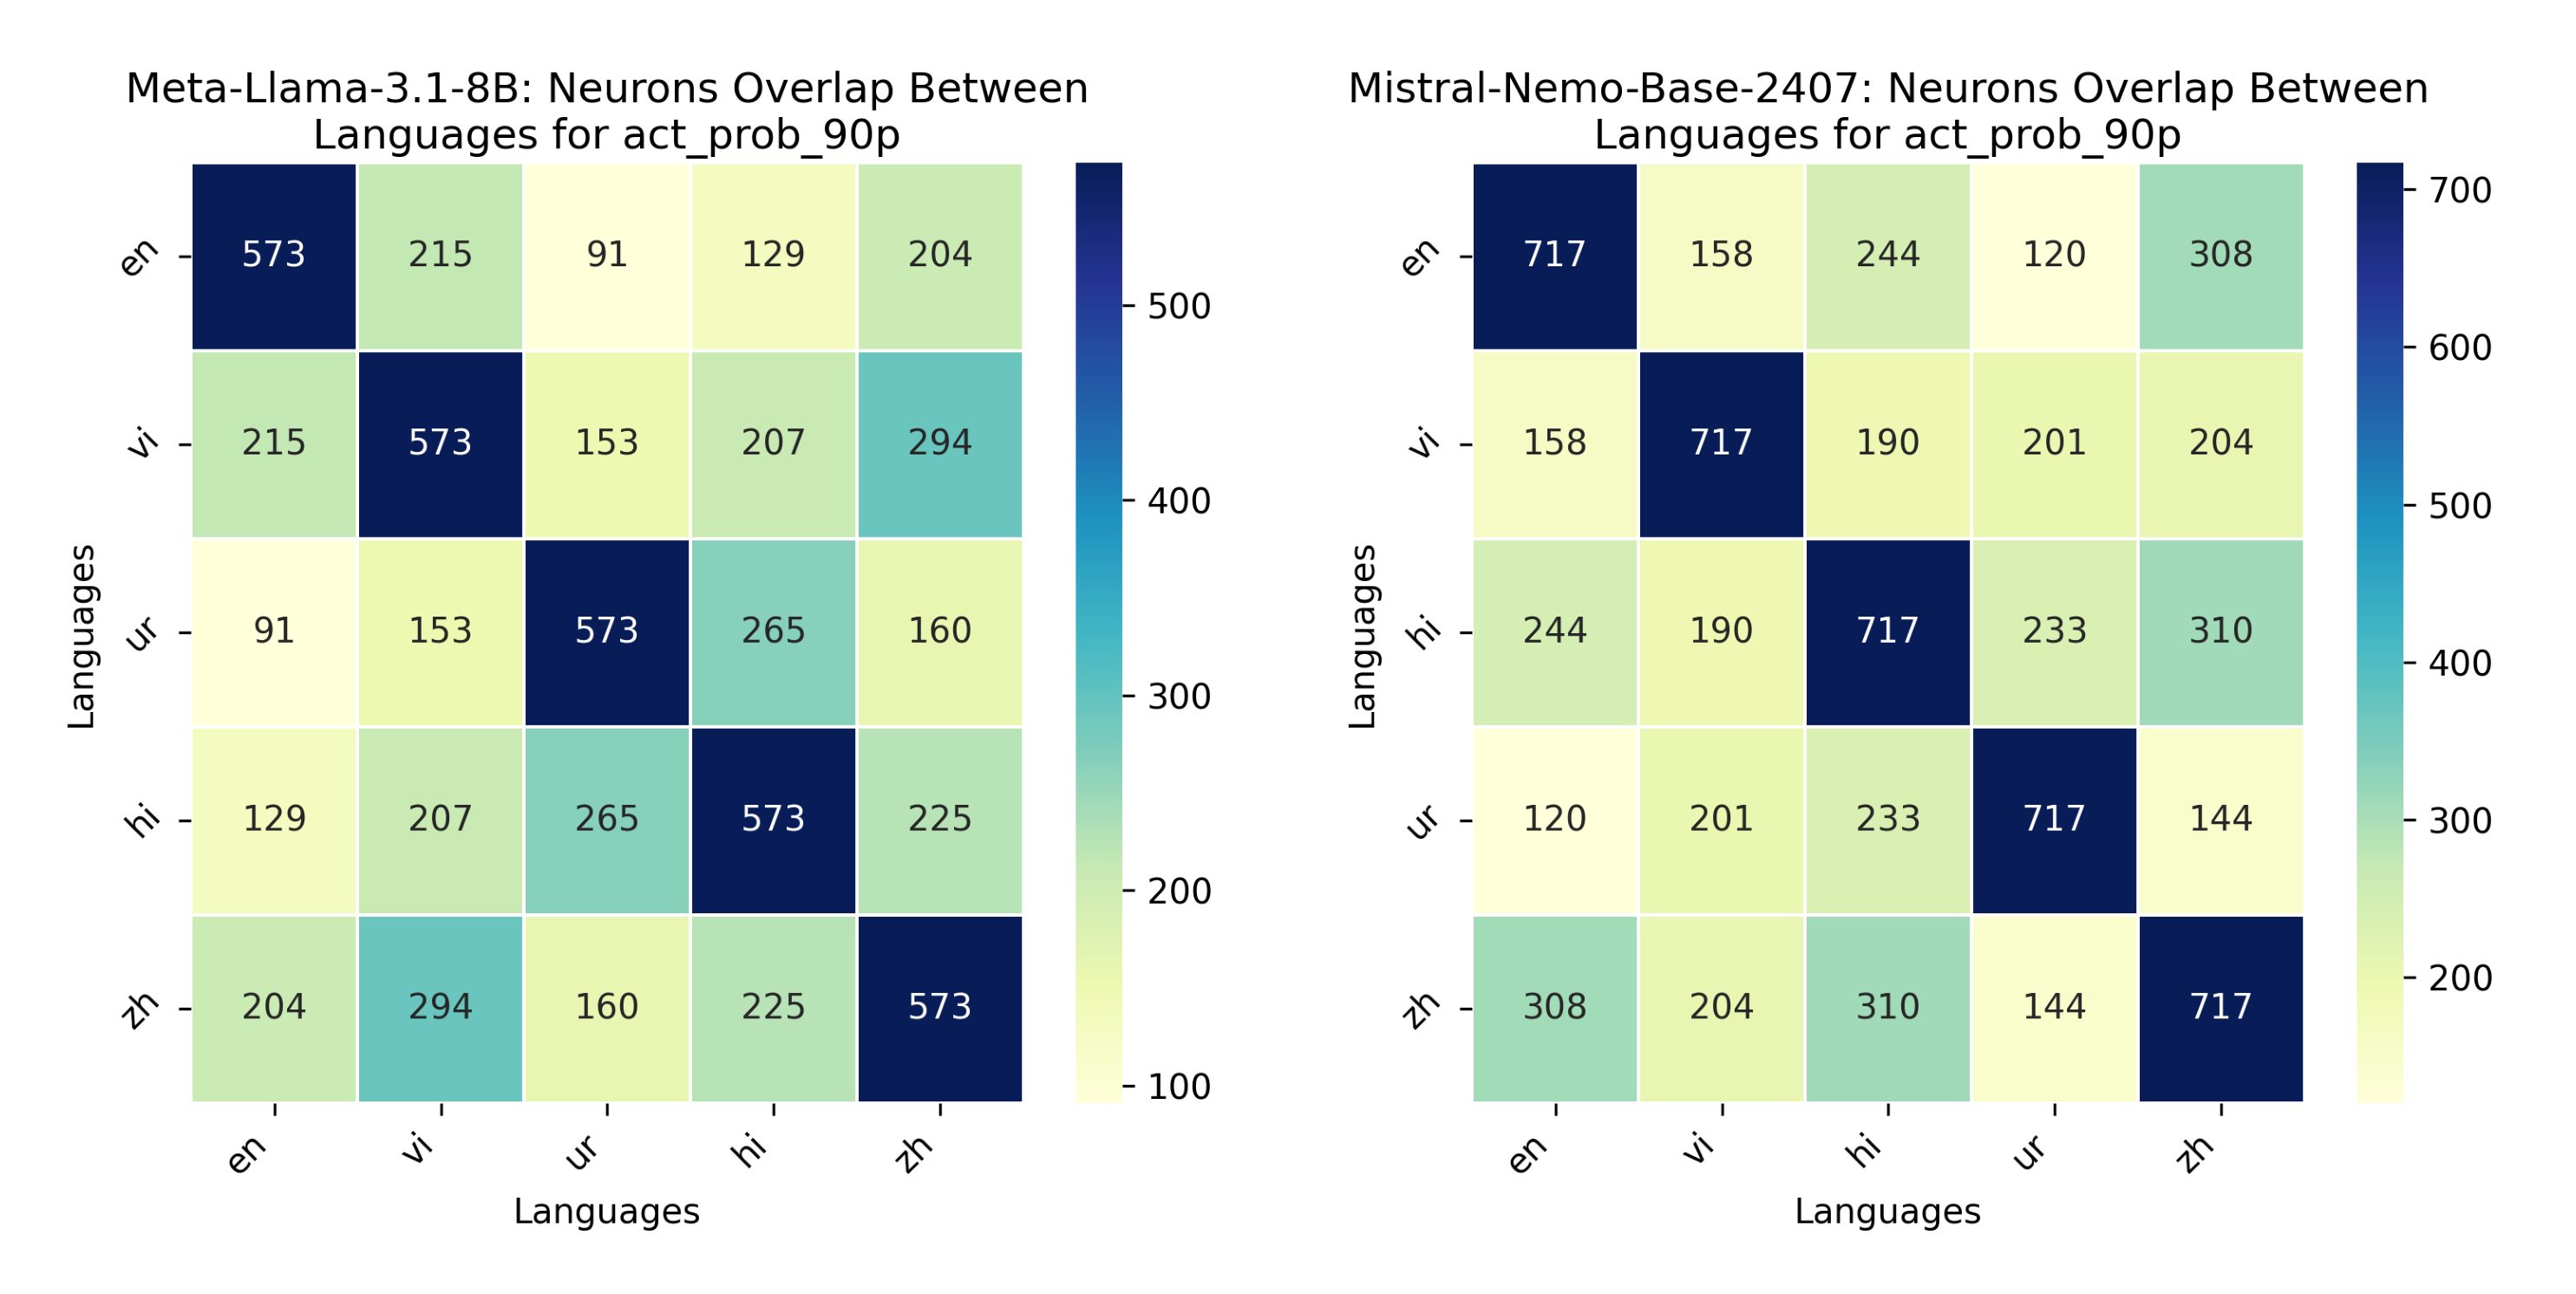
\includegraphics[width=0.8\linewidth]{Chapters/Chapter_3/figures/results/combined_act_lang_neurons_overlap.png}
	\caption{Overlap between the language-specific neuron sets under Act Prob 90p,
		for Llama~3.1 and Mistral Nemo. The diagonal is the size of each language's own
		set; the off-diagonal entries show that many neurons are shared across
		languages.}
	\label{fig:neurons-overlap-actprob}
\end{figure}

% FIGURE 3.5b (LAPE) -- include here.
% Suggested filename: fig_neuron_overlap_lape.png
% Content: pairwise neuron-set overlap heatmaps for LAPE, for Llama 3.1 and Mistral
% Nemo, on Set1 and Set6 (four panels).
\begin{figure}[ht]
	\centering
	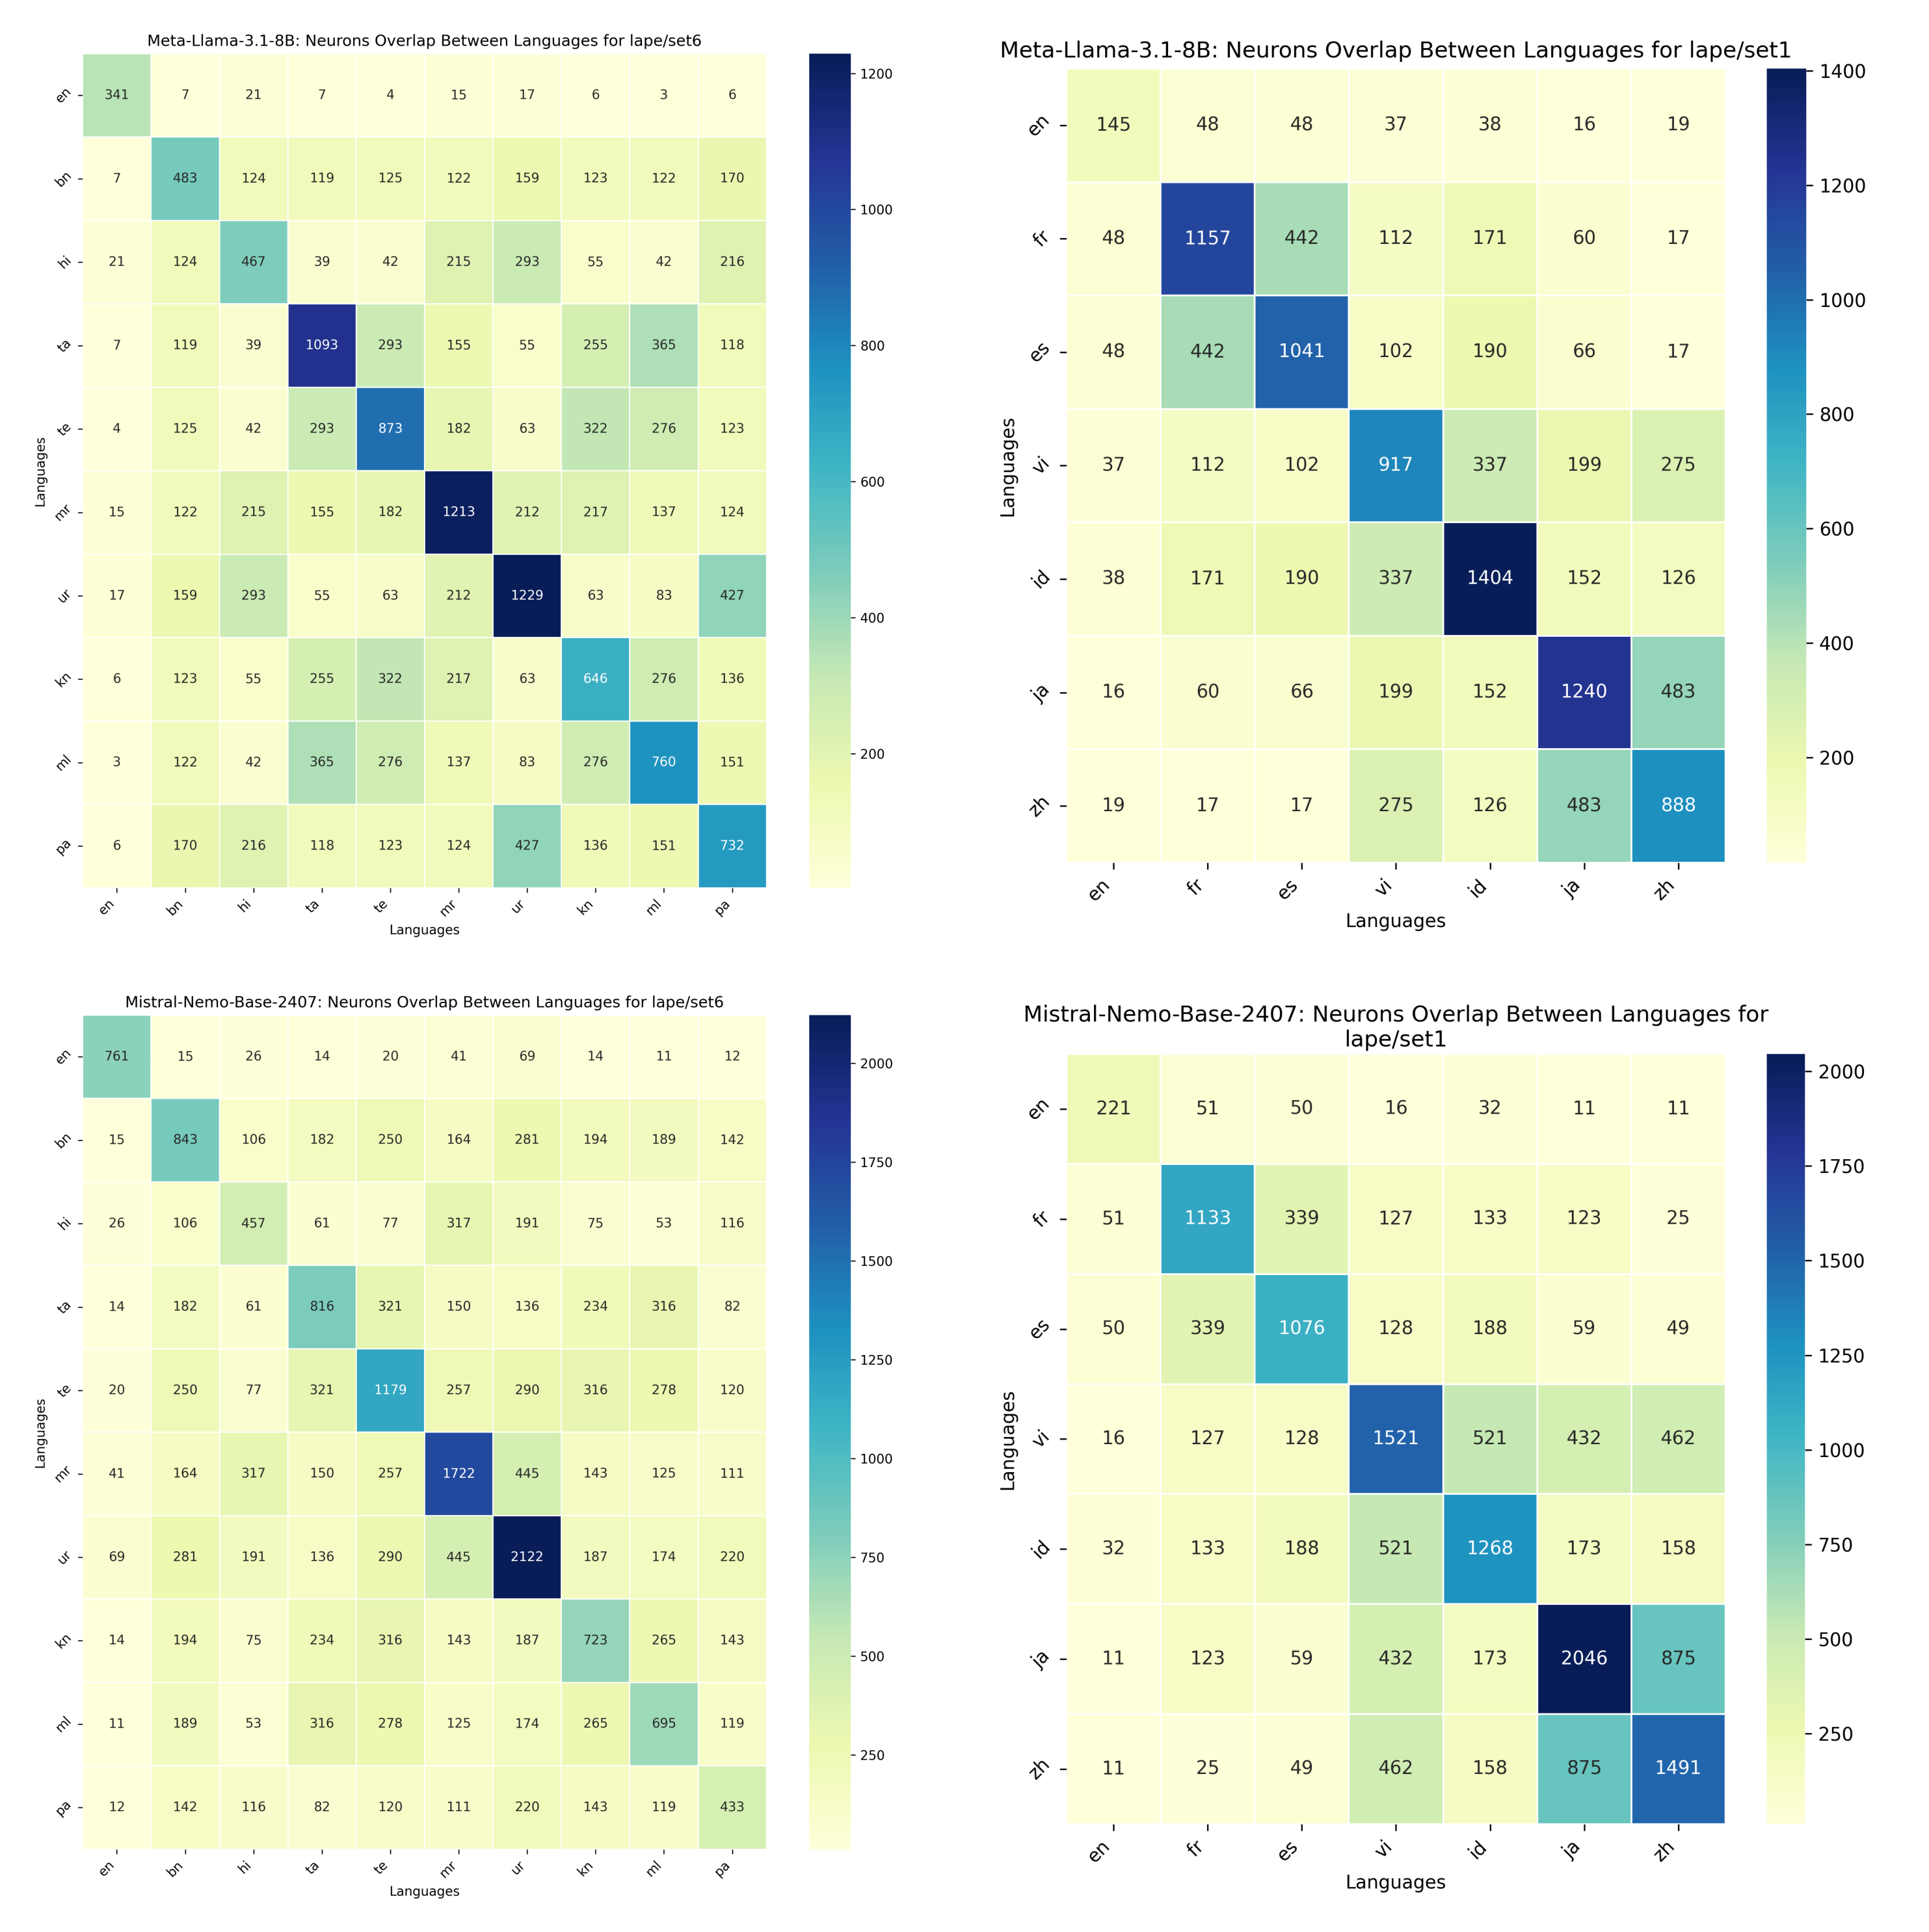
\includegraphics[width=0.8\linewidth]{Chapters/Chapter_3/figures/results/combined_lape_lang_neurons_overlap.png}
	\caption{Overlap between the language-specific neuron sets under LAPE, for
		Llama~3.1 and Mistral Nemo on Set1 and Set6. Related languages, such as Japanese
		and Chinese in Set1, share the most neurons.}
	\label{fig:neurons-overlap-lape}
\end{figure}

\subsection{Layer-Wise Distribution}
\label{subsec:neurons-layers}

We next look at where the identified neurons sit across the layers of the model.
Figure~\ref{fig:neurons-layers-lape} shows the distribution for LAPE, and
Figure~\ref{fig:neurons-layers-actprob} shows it for Act Prob 90p. The location of
the neurons depends on both the method and the model, and the two methods do not
agree.

Under LAPE, the neurons sit mostly in the upper part of the stack. For Llama~3.1
the counts are highest in the higher-middle layers, around layers 24 to 30, for
both Set1 and Set6. For Mistral Nemo the neurons concentrate in the topmost layers,
around layers 37 to 39, where the counts are much larger than anywhere else. The
bottom layers hold few neurons under LAPE, apart from a small number of isolated
cells.

Under Act Prob 90p the picture is different, and it also differs between the two
models. For Llama~3.1 the neurons are pushed towards the bottom of the stack: the
first layer holds a large number of English neurons, there is a strong band around
layers 3 and 4 across all languages, and the deeper layers stay sparse. For Mistral
Nemo the neurons sit in the middle of the stack, roughly layers 9 to 20, rather
than at either end, with the highest counts around layers 10 to 13 and layer 19.

So the two methods place language-specific neurons in different parts of the model,
and the layer pattern is not the same across the two models either. We point this
out because it matters for the discussion. As
Section~\ref{sec:neurons-results-transfer} shows, the two methods lead to the same
downstream conclusion even though they select neurons in different layers, which
means the result does not depend on where in the model the neurons are taken from.

% FIGURE 3.6a (LAPE) -- include here.
% Suggested filename: fig_neuron_layerwise_lape.png
% Content: layer-wise count of LAPE neurons per layer, for Llama 3.1 and Mistral
% Nemo, on Set1 and Set6 (four panels).
\begin{figure}[ht]
	\centering
	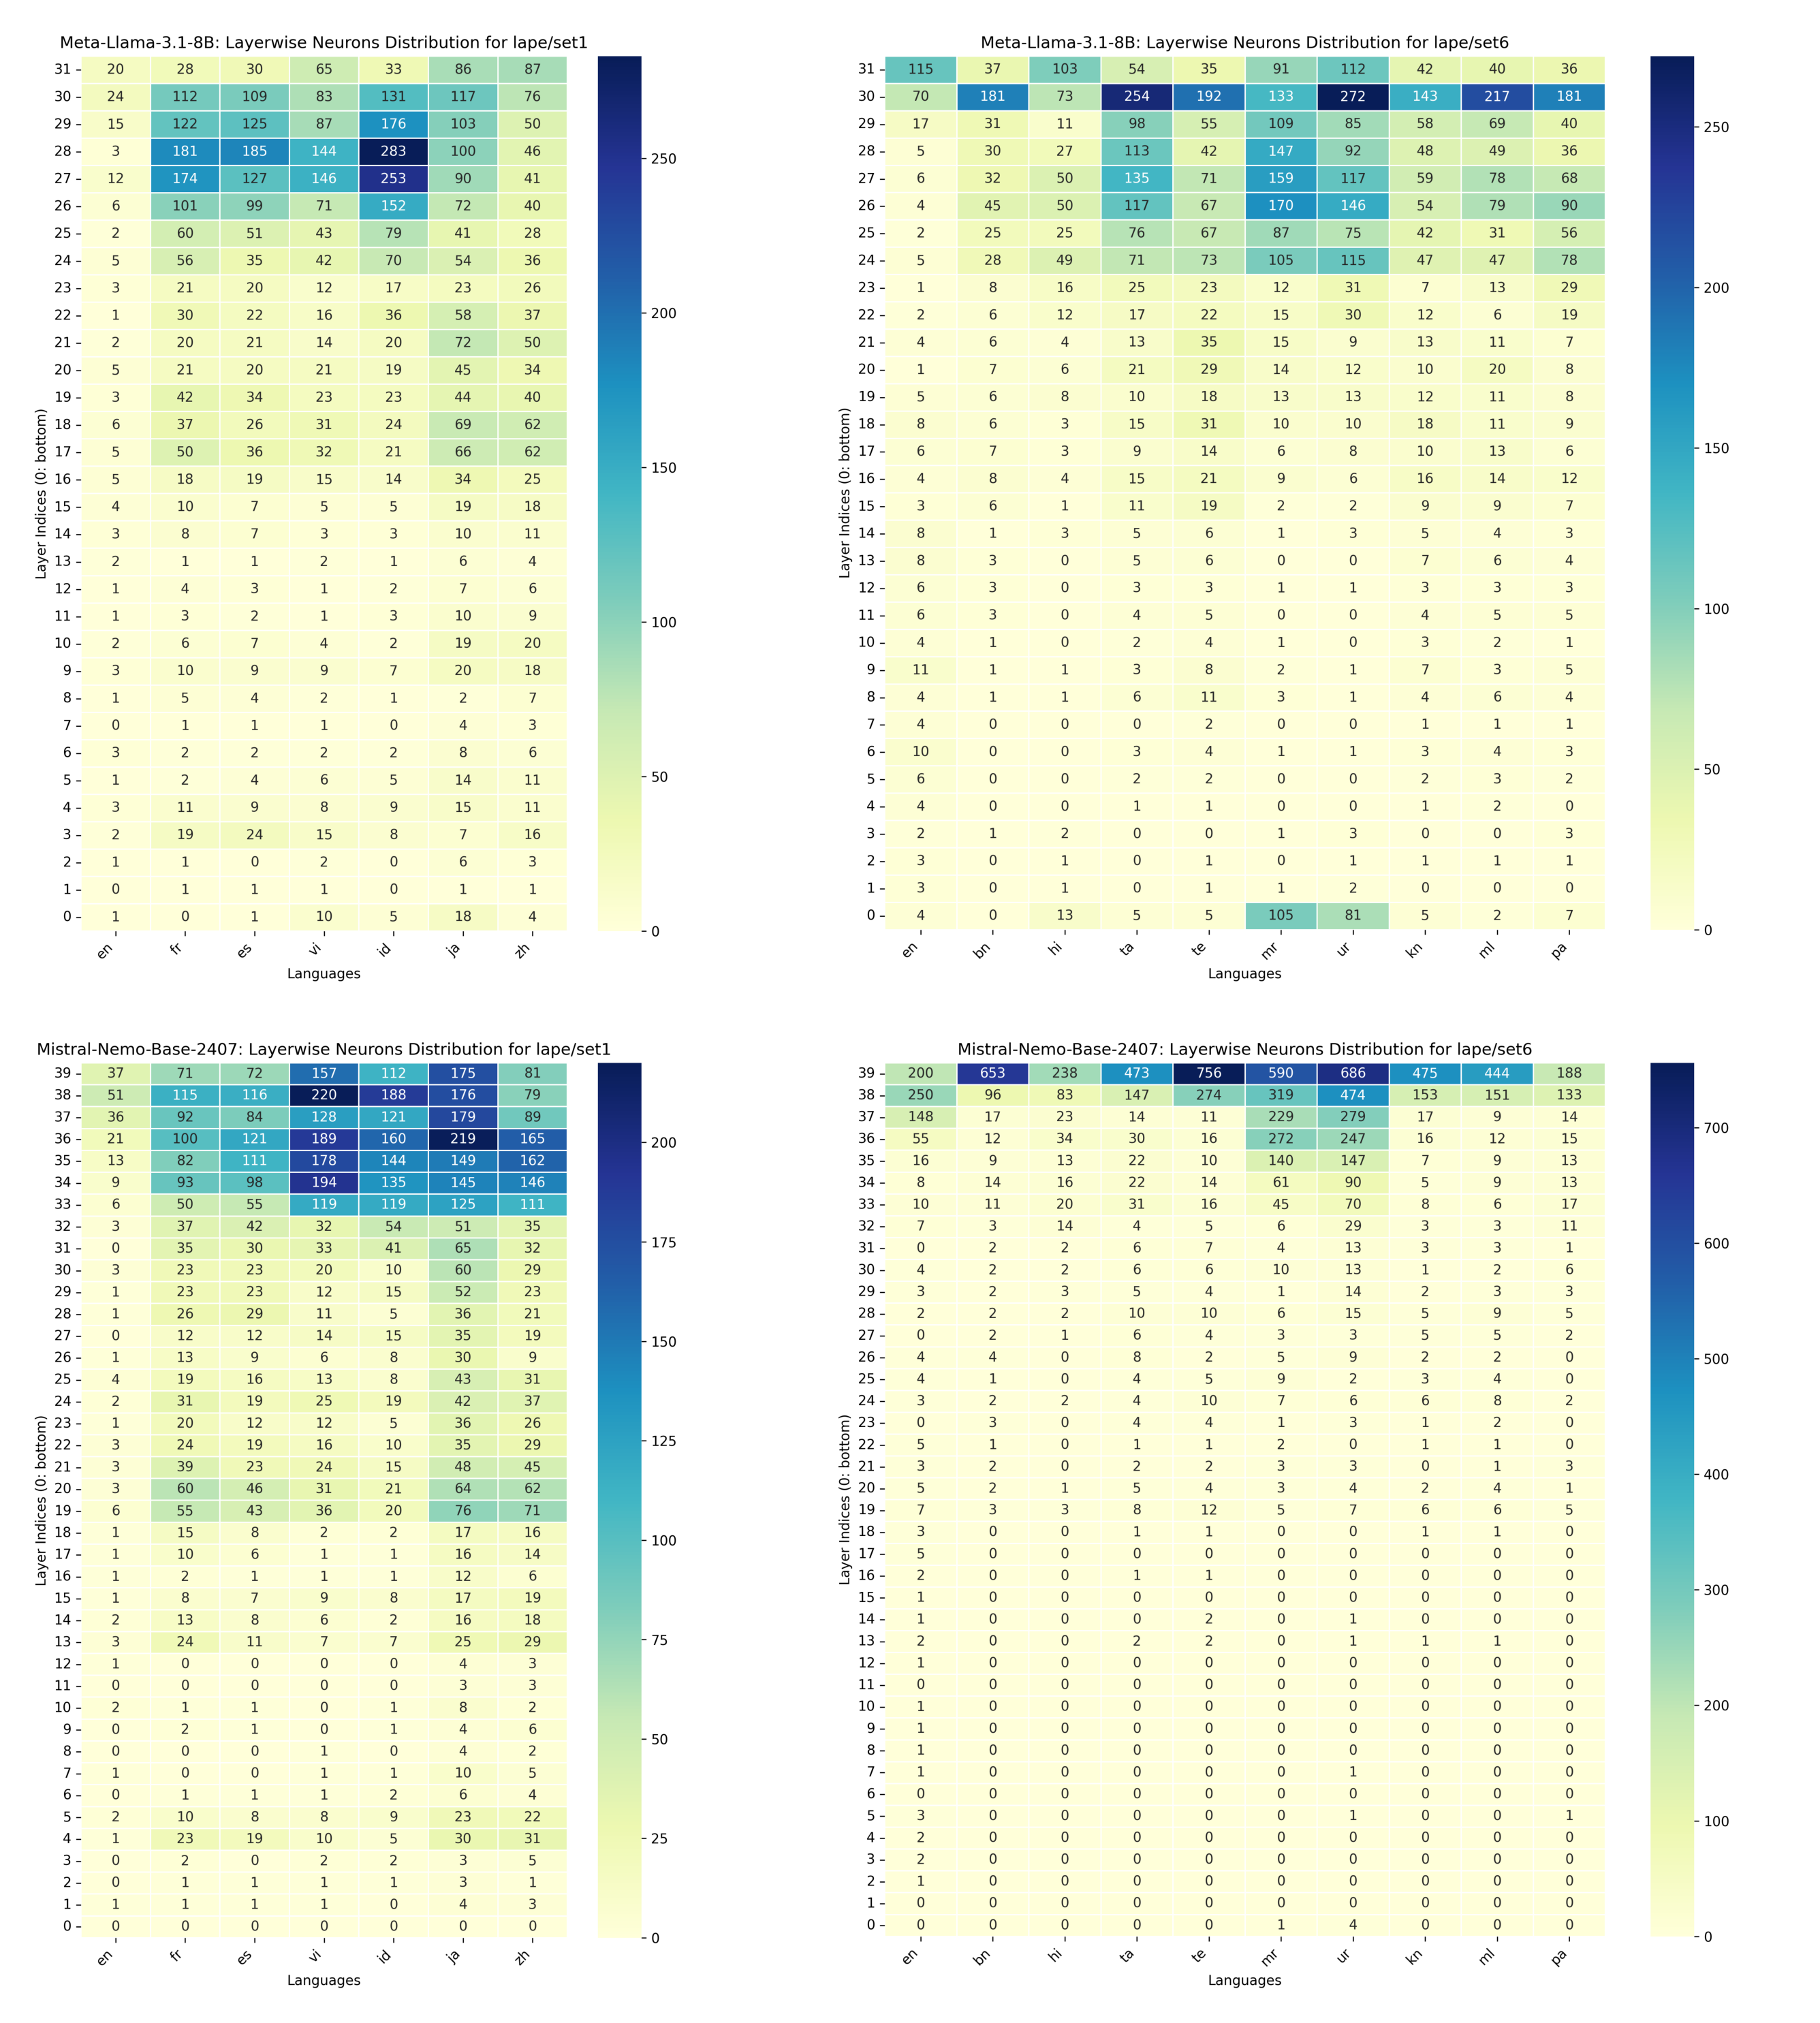
\includegraphics[width=0.8\linewidth]{Chapters/Chapter_3/figures/results/combined_lape_layerwise_lang_neurons_dist.png}
	\caption{Layer-wise distribution of language-specific neurons under LAPE, for
		Llama~3.1 and Mistral Nemo on Set1 and Set6. The neurons concentrate in the
		upper layers: the higher-middle layers for Llama~3.1 and the topmost layers for
		Mistral Nemo.}
	\label{fig:neurons-layers-lape}
\end{figure}

% FIGURE 3.6b (Act Prob 90p) -- include here.
% Suggested filename: fig_neuron_layerwise_actprob.png
% Content: layer-wise count of Act Prob 90p neurons per layer, for Llama 3.1 and
% Mistral Nemo.
\begin{figure}[ht]
	\centering
	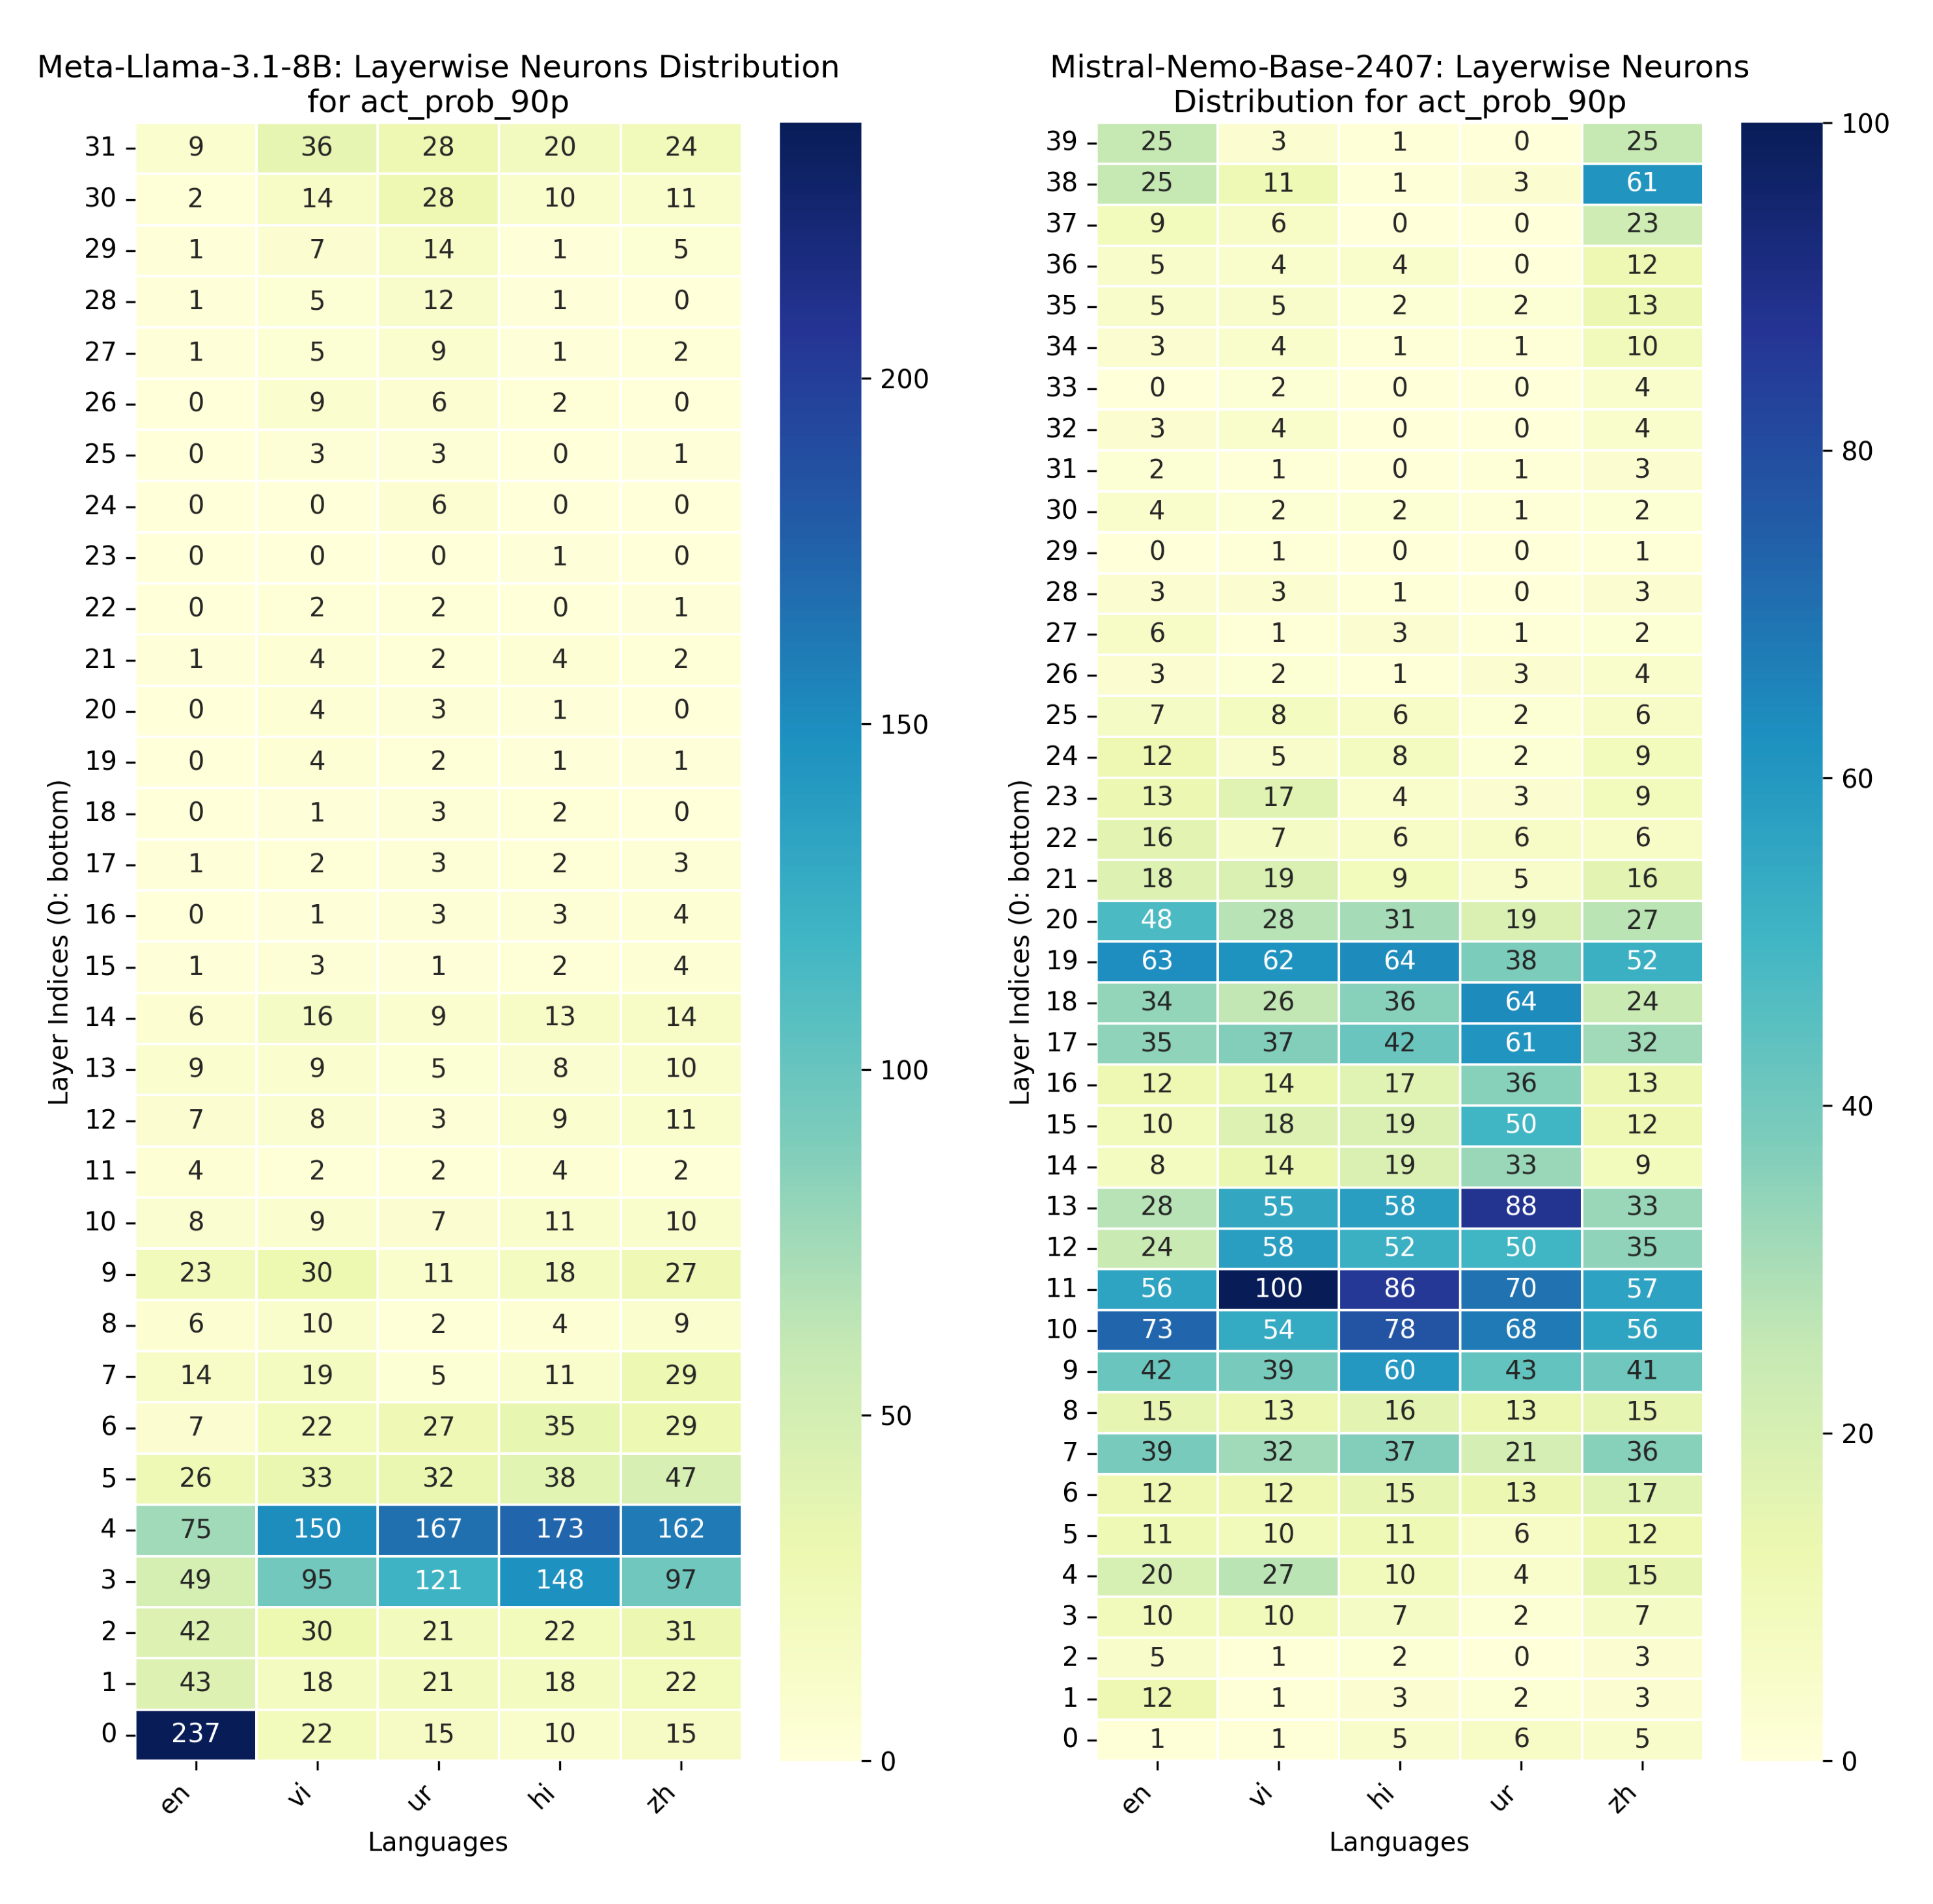
\includegraphics[width=0.8\linewidth]{Chapters/Chapter_3/figures/results/combined_act_layerwise_lang_neurons_dist.png}
	\caption{Layer-wise distribution of language-specific neurons under Act Prob
		90p, for Llama~3.1 and Mistral Nemo. The neurons sit at the bottom of the stack
		for Llama~3.1, with a large count in the first layer for English, and in the
		middle of the stack for Mistral Nemo.}
	\label{fig:neurons-layers-actprob}
\end{figure}

\subsection{Perplexity Change Under Intervention}
\label{subsec:neurons-ppxc-results}

We now check whether intervening on the neurons changes the model's handling of a
language, using the perplexity change of Equation~\ref{eq:neurons-ppxc}.
Figure~\ref{fig:neurons-ppxc} shows $\mathrm{PPXC}(i,j)$ as a heatmap, where row
$i$ is the language whose neurons are intervened on and column $j$ is the language
whose perplexity is measured. If the neurons were specific to their own language,
the diagonal ($i = j$) would be large and the off-diagonal entries small.

The heatmaps do not show this clean pattern. For most interventions the perplexity
change is small, including on the diagonal, which means that intervening on a
language's own neurons often does little to the model's perplexity on that
language. Where there are larger changes, they are not confined to the diagonal.
Setting activations to zero, in particular, does not produce the large diagonal
effect that would be expected if zero turned the neurons off. We take this up again
in the discussion, since it bears directly on the common practice of treating zero
as a way to deactivate a neuron.

% FIGURE 3.7 -- include here.
% Suggested filename: fig_ppxc_heatmap.pdf
% Content: PPXC heatmaps. Rows = language whose neurons are intervened on,
% columns = language whose perplexity is measured. Include the zero-intervention
% case (this is the publication's Figure 1) and, if available, the percentile
% cases, for LAPE and Act Prob 90p.
\begin{figure}[ht]
	\centering
	 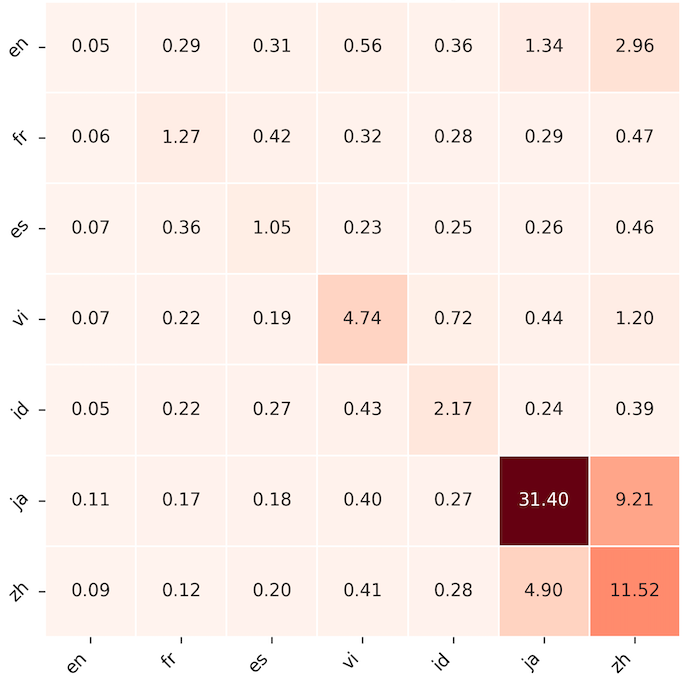
\includegraphics[width=0.6\linewidth]{Chapters/Chapter_3/figures/ppx.png}
	\caption{Perplexity change $\mathrm{PPXC}(i,j)$ under neuron intervention. Row
		$i$ is the language whose neurons are intervened on; column $j$ is the language
		whose perplexity is measured. Lower values mean the intervention has little
		effect. The changes are small for most interventions and are not concentrated
		on the diagonal.}
	\label{fig:neurons-ppxc}
\end{figure}

\section{Results: Cross-Lingual Transfer}
\label{sec:neurons-results-transfer}

We now turn to the main question, whether the interventions improve cross-lingual
task performance. We report results on XNLI and XQuAD, using English as the source
language and lower-resource languages as targets. For XNLI the target languages are
Vietnamese (vi), Hindi (hi), and Urdu (ur). For XQuAD they are Vietnamese (vi),
Hindi (hi), and Chinese (zh). In all settings the model is adapted using
English task data and evaluated on the target language without target-language task
data. The hyperparameters used for all fine-tuning runs are listed in
Table~\ref{tab:neurons-hyperparams}.

% TABLE 3.1 (hyperparameters) -- include here.
% Built from the published appendix (arXiv:2503.17456, App. B.2-B.3).
% Same settings apply to Llama 3.1 and Mistral Nemo; the only differences are
% per-task (XNLI vs XQuAD), so the table is organized by task.
\begin{table}[ht]
	\centering
	\begin{tabular}{lcc}
		\toprule
		\textbf{Setting} & \textbf{XNLI} & \textbf{XQuAD} \\
		\midrule
		\multicolumn{3}{l}{\textit{Models}} \\
		Backbones      & \multicolumn{2}{c}{Meta-Llama-3.1-8B, Mistral-Nemo-Base-2407} \\
		Quantization   & \multicolumn{2}{c}{4-bit (nf4), double quantization} \\
		Compute dtype  & \multicolumn{2}{c}{bfloat16} \\
		\midrule
		\multicolumn{3}{l}{\textit{LoRA}} \\
		Rank $r$              & 64    & 64    \\
		Scaling factor $\alpha$ & 128 & 128   \\
		\midrule
		\multicolumn{3}{l}{\textit{Optimization}} \\
		Optimizer          & AdamW & AdamW \\
		$\beta_1$, $\beta_2$ & 0.95, 0.999 & 0.95, 0.999 \\
		Learning rate      & $1\times10^{-6}$ & $5\times10^{-5}$ \\
		Weight decay       & 0.1   & 0.1   \\
		Gradient clipping  & 10.0  & 10.0  \\
		Warm-up            & 1\% of steps & 1\% of steps \\
		LR schedule        & linear decay & linear decay \\
		\midrule
		\multicolumn{3}{l}{\textit{Training}} \\
		Epochs             & 2     & 10    \\
		Batch size         & 8     & 4     \\
		Max context length & 256   & 512   \\
		Train split used   & 25\%  & 100\% \\
		Eval split used    & 100\% & 100\% \\
		\bottomrule
	\end{tabular}
	\caption{Hyperparameters for neuron-targeted fine-tuning on XNLI and XQuAD. The
		same settings are used for Llama~3.1 and Mistral Nemo; values differ only
		between the two tasks.}
	\label{tab:neurons-hyperparams}
	\end{table}

\subsection{Baseline}
\label{subsec:neurons-baseline}

Before applying any intervention, we record the no-intervention performance of each
model, which is the zero-shot cross-lingual transfer after adaptation on English
with no neuron edited. Table~\ref{tab:neurons-baseline} reports these numbers. They
are the reference for the rest of the section: an intervention is only useful if it
improves on this baseline. For XNLI we report accuracy on Vietnamese, Hindi, and
Urdu; for XQuAD we report exact match and, in parentheses, F1 on Vietnamese, Hindi,
and Chinese.

% TABLE 3.2 (baseline) -- include here.
% Built from the "No Int" column of the full XNLI and XQuAD result tables.
\begin{table}[ht!]
	\centering
	\renewcommand{\arraystretch}{1.2}
	\begin{tabular}{llcc}
		\toprule
		\textbf{Model} & \textbf{Eval Lang} & \textbf{XNLI (Acc \%)} & \textbf{XQuAD (EM (F1))} \\
		\midrule
		\multirow{3}{*}{Llama 3.1}   & vi      & 80.5 & 41 (73.5) \\
		& hi      & 75.0 & 38 (64.1) \\
		& ur / zh & 70.0 & 56 (77.5) \\
		\midrule
		\multirow{3}{*}{Mistral Nemo} & vi      & 80.5 & 39 (74.6) \\
		& hi      & 76.1 & 38 (66.9) \\
		& ur / zh & 66.8 & 47 (74.9) \\
		\bottomrule
	\end{tabular}
	\caption{No-intervention (zero-shot transfer) results for Llama~3.1 and Mistral Nemo. XNLI evaluates on vi/hi/ur (accuracy); XQuAD on vi/hi/zh (exact match with F1 in parentheses).}
	\label{tab:neurons-baseline}
\end{table}

\subsection{Test-Time Interventions}
\label{subsec:neurons-testtime-results}

Tables~\ref{tab:neurons-xnli-testtime} and~\ref{tab:neurons-xquad-testtime} report
the test-time intervention results on XNLI and XQuAD. In each table the baseline is
the No Int column, and the remaining columns replace the language-specific neuron
activations with the mean, with higher percentiles ($P75$, $P90$, $P95$), with
zero, and with lower percentiles ($P5$, $P10$, $P25$), for both identification
methods.

The main point is that no intervention improves the target languages as a group.
On XNLI, the best column for most rows is No Int, and where an intervention edges
above the baseline the gain is small, for example Llama~3.1 with LAPE on Hindi and
Urdu, where the mean intervention adds about two tenths of a point. These small
gains do not carry across languages or across the two models, so they read as noise
rather than a real effect.

The interventions do not only fail to help, they often hurt, and the size of the
damage depends on the model, the task, and the replacement value. For Llama~3.1 the
changes on XNLI stay within a few points. For Mistral Nemo they are much larger: the
lower-percentile and zero settings can pull accuracy down sharply, and with
Act~Prob~90p the $P5$ setting on Vietnamese drops from $80.5$ to the high thirties.
The lower percentiles are the most destructive overall, which fits the idea that
forcing these neurons to a low value disturbs computations the task depends on.

XQuAD shows the same pattern more strongly. The scores swing widely across
intervention columns, and several settings collapse the model: the mean
intervention takes Llama~3.1 with LAPE on Chinese from $56$ exact match to $10$,
and for Mistral~Nemo the higher-percentile and low-percentile settings drive
exact match to $0$ on some languages. As on XNLI, No Int is at or near the best
column for most rows, and no intervention lifts the three target languages together.

Setting the activations to zero is worth singling out, since zeroing is often used
as a way to switch a neuron off. The Int~0 column does not behave like removing a
needed component. On XNLI it stays close to the baseline in most rows, and on XQuAD
it is sometimes among the better intervention columns rather than the worst. This
matches the perplexity result in Section~\ref{subsec:neurons-ppxc-results}: zero is
just another value these activations can take, not an off state. The two
identification methods, LAPE and Act~Prob~90p, lead to the same overall picture, so
the outcome does not depend on how the neurons are chosen.

% TABLE 3.3 (XNLI test-time) -- paste the full XNLI intervention table here,
% converted to booktabs (toprule/midrule/bottomrule, no vertical bars).
% Label: tab:neurons-xnli-testtime
\begin{table}[t]
	\centering
	\renewcommand{\arraystretch}{1.2}
	\setlength{\tabcolsep}{5pt}
	\begin{small}
		\begin{tabular}{llcccccccc}
			\toprule
			\textbf{Model \& Method} & \textbf{Lang} & \textbf{No Int} & \textbf{Int} $\bm{\mu}$ & \textbf{P75} & \textbf{P90} & \textbf{P95} & \textbf{Int 0} & \textbf{P5} & \textbf{P10} \\
			\midrule
			\multirow{3}{*}{Llama 3.1 + LAPE}
			& vi & \textbf{80.5} & 79.5 & 79.1 & 79.0 & 78.9 & 79.8 & 73.6 & 77.7 \\
			& hi & 75.0 & \textbf{75.2} & 74.9 & 74.9 & 75.0 & 74.4 & 74.8 & 75.1 \\
			& ur & 70.0 & \textbf{70.4} & 70.2 & 69.3 & 69.0 & 68.5 & 68.6 & 68.7 \\
			\midrule
			\multirow{3}{*}{Llama 3.1 + Act Prob 90p}
			& vi & \textbf{80.5} & 78.2 & 78.9 & 79.3 & 79.5 & 79.0 & 76.5 & 77.4 \\
			& hi & \textbf{75.0} & 74.1 & 72.6 & 71.8 & 71.2 & 73.7 & 75.0 & 74.6 \\
			& ur & \textbf{70.0} & 69.7 & 69.7 & 69.3 & 68.7 & 69.6 & 69.4 & 69.5 \\
			\midrule
			\multirow{3}{*}{Mistral Nemo + LAPE}
			& vi & 80.5 & 80.4 & 80.5 & \textbf{80.6} & 80.5 & 79.2 & \textbf{80.6} & 80.5 \\
			& hi & \textbf{76.1} & 69.8 & 67.8 & 66.9 & 66.6 & 74.9 & 73.0 & 72.4 \\
			& ur & 66.8 & 66.5 & 67.2 & 67.0 & 66.8 & \textbf{66.9} & 65.8 & 65.4 \\
			\midrule
			\multirow{3}{*}{Mistral Nemo + Act Prob 90p}
			& vi & 80.5 & 67.4 & 79.0 & \textbf{81.1} & \textbf{81.1} & 79.8 & 37.4 & 40.7 \\
			& hi & \textbf{76.1} & 72.2 & 73.7 & 74.5 & 74.4 & 74.5 & 62.4 & 66.3 \\
			& ur & \textbf{66.8} & 65.9 & 64.0 & 61.3 & 59.7 & 66.4 & 54.6 & 61.6 \\
			\bottomrule
		\end{tabular}
	\end{small}
	\caption{XNLI test-time intervention accuracy. No Int is the baseline; the other
		columns set the language-specific neuron activations to the mean, to higher
		percentiles, to zero, and to lower percentiles, for LAPE and Act Prob 90p. The
		best value in each row is in bold. No intervention improves the three target
		languages as a group, and the lower-percentile and zero settings often degrade
		accuracy, most clearly for Mistral Nemo.}
	\label{tab:neurons-xnli-testtime}
\end{table}

% TABLE 3.4 (XQuAD test-time) -- paste the full XQuAD intervention table here,
% converted to booktabs. Each cell is EM (F1). Label: tab:neurons-xquad-testtime
\begin{table}[t]
	\centering
	\renewcommand{\arraystretch}{1.3}
	\setlength{\tabcolsep}{3.5pt}
	\begin{scriptsize}
		\begin{tabular}{llcccccccc}
			\toprule
			\textbf{Model \& Method} & \textbf{Lang} & \textbf{No Int} & \textbf{Int} $\bm{\mu}$ & \textbf{P75} & \textbf{P90} & \textbf{P95} & \textbf{Int 0} & \textbf{P5} & \textbf{P10} \\
			\midrule
			\multirow{3}{*}{Llama 3.1 + LAPE}
			& vi & 41 (73.5) & 40 (72.9) & 36 (76.7) & 31 (69.5) & 28 (66.8) & 32 (69.2) & 4 (35.8) & 10 (43.2) \\
			& hi & 38 (64.1) & 40 (65.5) & 38 (66.4) & 36 (65.4) & 36 (66.3) & 23 (49.9) & 38 (62.8) & 37 (62.8) \\
			& zh & 56 (77.5) & 10 (62.8) & 3 (58.1) & 3 (56.1) & 4 (52.9) & 33 (63.2) & 20 (49.1) & 33 (63.2) \\
			\midrule
			\multirow{3}{*}{Llama 3.1 + Act Prob 90p}
			& vi & 41 (73.6) & 39 (73.0) & 26 (65.8) & 23 (64.9) & 24 (64.8) & 42 (73.8) & 33 (67.8) & 36 (70.3) \\
			& hi & 38 (64.1) & 34 (60.7) & 35 (62.3) & 36 (62.8) & 32 (61.9) & 38 (62.9) & 23 (54.9) & 31 (58.6) \\
			& zh & 56 (77.5) & 61 (80.7) & 59 (79.5) & 56 (78.8) & 56 (78.4) & 55 (78.5) & 40 (61.7) & 50 (73.6) \\
			\midrule
			\multirow{3}{*}{Mistral Nemo + LAPE}
			& vi & 39 (74.6) & 42 (76.8) & 40 (76.4) & 40 (75.0) & 39 (73.6) & 13 (45.0) & 10 (40.4) & 11 (41.2) \\
			& hi & 38 (66.9) & 35 (65.9) & 38 (67.1) & 37 (66.6) & 34 (66.5) & 22 (51.7) & 36 (65.8) & 36 (66.1) \\
			& zh & 47 (74.9) & 24 (74.0) & 4 (65.6) & 0 (61.6) & 0 (59.3) & 14 (53.3) & 1 (33.6) & 24 (68.9) \\
			\midrule
			\multirow{3}{*}{Mistral Nemo + Act Prob 90p}
			& vi & 39 (74.6) & 11 (43.3) & 26 (62.8) & 29 (63.9) & 15 (48.5) & 39 (74.5) & 0 (3.8) & 0 (6.5) \\
			& hi & 38 (66.9) & 26 (54.4) & 34 (65.1) & 37 (68.9) & 37 (68.7) & 33 (63.8) & 0 (6.0) & 0 (11.9) \\
			& zh & 47 (74.9) & 46 (77.4) & 26 (69.9) & 20 (59.8) & 15 (54.9) & 48 (76.2) & 0 (8.5) & 0 (17.0) \\
			\bottomrule
		\end{tabular}
	\end{scriptsize}
	\caption{XQuAD test-time intervention results, reported as exact match with F1
		in parentheses, for the same intervention columns as
		Table~\ref{tab:neurons-xnli-testtime}. The pattern matches XNLI but the swings
		are larger: several settings collapse the score, such as Llama~3.1 with LAPE on
		Chinese under the mean intervention and Mistral~Nemo under the higher- and
		lower-percentile settings. No intervention lifts the three target languages
		together.}
	\label{tab:neurons-xquad-testtime}
\end{table}

\subsection{Neuron Fine-Tuning}
\label{subsec:neurons-ft}

The test-time interventions in
Section~\ref{subsec:neurons-testtime-results} fixed the neuron activations to a
chosen value. Here we instead fine-tune the identified neurons, so the model can
adjust them through training rather than having them set by hand.
Table~\ref{tab:neurons-ft} reports this for Llama~3.1 on XNLI, for both
identification methods and under the three fine-tuning-language (FTL) settings from
Section~\ref{subsec:neurons-config}: fine-tuning the source-language (English)
neurons, the target-language neurons, or both. The task training data is always
English. For each fine-tuned model we also apply the test-time interventions, so
each row shows the no-intervention score next to the mean, $P90$, zero, and $P10$
settings.

Two things stand out. First, for Vietnamese and Hindi the no-intervention column is
the best or close to the best in every row, for both LAPE and Act~Prob~90p.
Fine-tuning the neurons and then intervening on them does not beat simply
fine-tuning and leaving the neurons alone. Second, the choice of which language's
neurons are made trainable barely changes the result. Within a target language the
three FTL settings give almost the same scores, for example Vietnamese stays near
$80.1$ under LAPE whether we fine-tune the English neurons, the Vietnamese neurons,
or both. If the language-specific neurons carried information that transfers to the
target language, we would expect fine-tuning the target-language neurons to help
more than fine-tuning the English ones, and we do not see that.

The one place any column edges above the baseline is Urdu, where the mean
intervention reaches about $70.4$ to $70.6$ against a baseline near $70.0$. This is
a fraction of a point, it appears only for one language, and it does not hold for
Vietnamese or Hindi, so it is not evidence that the approach works. The pattern is
the same under Act~Prob~90p as under LAPE. Since Act~Prob~90p does not depend on the
choice of language set, while LAPE does, the agreement between the two also rules
out the language-set normalization in LAPE as the reason for the negative result.
Overall the fine-tuning experiment points the same way as the test-time one: acting
on the identified neurons does not improve cross-lingual transfer.

% TABLE 3.5 (neuron fine-tuning, XNLI, Llama 3.1) -- booktabs style, no vertical
% bars. LAPE and Act Prob 90p in one table, split by section rows.
% Label: tab:neurons-ft
\begin{table}[ht!]
	\centering
	\renewcommand{\arraystretch}{1.15}
	\setlength{\tabcolsep}{6pt}
	\footnotesize
	\begin{tabular}{llccccc}
		\toprule
		\textbf{FTL} & \textbf{EL} & \textbf{No Int} & \textbf{Int} $\bm{\mu}$ & \textbf{Int P90} & \textbf{Int 0} & \textbf{Int P10} \\
		\midrule
		\multicolumn{7}{c}{\textit{Llama 3.1 with LAPE}} \\
		\midrule
		en     & vi & \textbf{80.2} & 79.6 & 78.5 & 79.2 & 78.0 \\
		vi     & vi & \textbf{80.1} & 79.5 & 78.6 & 79.2 & 78.0 \\
		en+vi  & vi & \textbf{80.1} & 79.4 & 78.5 & 79.1 & 78.0 \\
		\midrule
		en     & hi & \textbf{74.9} & 74.6 & 74.6 & 74.1 & 74.6 \\
		hi     & hi & \textbf{74.9} & 74.6 & 74.5 & 74.3 & 74.6 \\
		en+hi  & hi & \textbf{74.9} & 74.5 & 74.5 & 74.3 & 74.7 \\
		\midrule
		en     & ur & 69.8 & \textbf{70.4} & 69.6 & 70.2 & 69.0 \\
		ur     & ur & \textbf{69.8} & 70.5 & 69.5 & 70.4 & 69.1 \\
		en+ur  & ur & 70.0 & \textbf{70.6} & 69.5 & 70.3 & 68.9 \\
		\midrule
		\multicolumn{7}{c}{\textit{Llama 3.1 with Act Prob 90p}} \\
		\midrule
		en     & vi & \textbf{80.3} & 78.0 & 79.1 & 78.5 & 77.5 \\
		vi     & vi & \textbf{80.1} & 78.0 & 79.0 & 78.7 & 77.4 \\
		en+vi  & vi & \textbf{80.1} & 78.0 & 78.9 & 78.8 & 77.4 \\
		\midrule
		en     & hi & \textbf{74.9} & 73.9 & 72.1 & 73.3 & 74.5 \\
		hi     & hi & \textbf{74.9} & 73.8 & 72.1 & 73.9 & 74.6 \\
		en+hi  & hi & \textbf{74.9} & 73.7 & 72.1 & 73.8 & 74.6 \\
		\midrule
		en     & ur & 69.9 & \textbf{70.1} & 69.4 & 70.0 & 69.5 \\
		ur     & ur & 69.9 & 70.0 & 69.4 & \textbf{70.1} & 69.5 \\
		en+ur  & ur & 69.8 & 69.9 & 69.3 & \textbf{70.1} & 69.6 \\
		\bottomrule
	\end{tabular}
	\caption{Neuron fine-tuning results for Llama~3.1 on XNLI, for LAPE and
		Act~Prob~90p. FTL is the fine-tuning language (English, the target, or both);
		EL is the evaluation language; task training data is always English. Each
		fine-tuned model is also evaluated under the test-time interventions (mean,
		$P90$, zero, $P10$). The best value in each row is in bold. No~Int is the best
		column in nearly every row, and the FTL setting has little effect, so
		fine-tuning the identified neurons does not improve cross-lingual transfer.}
	\label{tab:neurons-ft}
\end{table}

\subsection{Random-Neuron Control}
\label{subsec:neurons-random}

The interventions so far act on neurons that a method marked as language-specific.
A natural question is whether these neurons matter more than any other neurons. To
check this, we run a control in which we fine-tune randomly chosen neurons instead
of the identified ones, keeping the number of fine-tuned neurons the same (ten per
layer). Everything else, including the English task training and the evaluation
setup, is unchanged. Table~\ref{tab:neurons-random} reports the zero-shot
(No~Int) accuracy after this random-neuron fine-tuning.

The scores are close to those from fine-tuning the language-specific neurons in
Table~\ref{tab:neurons-ft}. For Llama~3.1, random-neuron fine-tuning gives $80.1$
on Vietnamese, $74.8$ on Hindi, and $69.8$ on Urdu, which are within a fraction of
a point of the corresponding language-specific runs. If the identified neurons
carried information that ordinary neurons did not, fine-tuning them should beat
fine-tuning random ones, and we do not see that gap. This is what we would expect
if the selected neurons are not doing anything special for the task that other
neurons cannot also do, and it fits the overlap and polysemanticity results
discussed earlier. The control therefore supports the same conclusion as the rest
of the section: the negative result is not because we picked the wrong neurons, but
because acting on a small set of neurons, identified or random, does not change
cross-lingual transfer.

% TABLE 3.6 (random-neuron control) -- booktabs style, no vertical bars.
% Label: tab:neurons-random
\begin{table}[ht!]
	\centering
	\renewcommand{\arraystretch}{1.3}
	\setlength{\tabcolsep}{8pt}
	\footnotesize
	\begin{tabular}{llcc}
		\toprule
		\textbf{Model} & \textbf{FTL} & \textbf{EL} & \textbf{No Int} \\
		\midrule
		\multirow{3}{*}{Llama 3.1}    & rand & vi & 80.1 \\
		& rand & hi & 74.8 \\
		& rand & ur & 69.8 \\
		\midrule
		\multirow{3}{*}{Mistral Nemo} & rand & vi & 80.4 \\
		& rand & hi & 75.6 \\
		& rand & ur & 65.5 \\
		\bottomrule
	\end{tabular}
	\caption{Random-neuron control. Zero-shot (No~Int) XNLI accuracy after
		fine-tuning ten randomly selected neurons per layer, instead of the
		language-specific neurons, for Llama~3.1 and Mistral~Nemo. The scores are close
		to the language-specific fine-tuning results in
		Table~\ref{tab:neurons-ft}, so the identified neurons are not doing something
		other neurons cannot.}
	\label{tab:neurons-random}
\end{table}

\section{Discussion}
\label{sec:neurons-discussion}

The results are consistent in their conclusion across tasks, models, and
identification methods: interventions on language-specific neurons do not give a
reliable improvement in cross-lingual task performance. This section discusses why.

\subsection{Polysemantic Neurons and Entangled Function}
\label{subsec:neurons-polysemantic}

The neuron analysis points to one explanation. The identified neurons are shared
across languages (Section~\ref{subsec:neurons-overlap}), and the random-neuron
control (Section~\ref{subsec:neurons-random}) gives almost the same scores as
fine-tuning the identified neurons, so the selected neurons are not doing anything
that other neurons cannot. This fits the idea that a single neuron takes part in
more than one function, often called polysemanticity
\citep{elhage2022superposition}. If a neuron contributes to several computations at
once, including ones the task depends on, then fixing its activation or restricting
fine-tuning to it disturbs those other computations as well. The intervention is
not surgical, even though the neuron was selected as language-specific.

\subsection{Zero Is Not Deactivation}
\label{subsec:neurons-zero}

A common way to test a neuron's role is to set its activation to zero and see what
breaks. Our results show this is not a safe assumption here. Setting the activations
to zero does not produce a large perplexity change
(Section~\ref{subsec:neurons-ppxc-results}), and the Int~0 column does not collapse
task performance the way removing a needed component would
(Section~\ref{subsec:neurons-testtime-results}); on XQuAD it is sometimes among the
better intervention columns rather than the worst. For these activations, zero is
just another value the neuron can take, not an off state. Conclusions that rely on
zeroing a neuron to measure its importance should be treated with care.

\subsection{Neurons Are Not Independent Across Languages}
\label{subsec:neurons-independence}

The overlap between the language sets
(Section~\ref{subsec:neurons-overlap}) and the off-diagonal perplexity changes
(Section~\ref{subsec:neurons-ppxc-results}) both show that the neurons for one
language are tied to those of others. This matters for the original goal. The
appeal of language-specific neurons was that one could improve a target language by
acting on its own neurons. If those neurons are shared with other languages, there
is no clean handle to act on, and an edit aimed at one language reaches the others
as well.

\subsection{The Result Does Not Depend on How Neurons Are Selected}
\label{subsec:neurons-consistency}

LAPE and Act~Prob~90p score and select neurons differently. They also place the
selected neurons in different parts of the model: as the layer-wise and overlap
results show (Section~\ref{subsec:neurons-layers},
Section~\ref{subsec:neurons-overlap}), LAPE concentrates neurons in the upper
layers while Act~Prob~90p places them at the bottom for Llama~3.1 and in the middle
for Mistral~Nemo, and the two methods select largely different sets. Despite this,
they lead to the same downstream conclusion in every experiment. The fact that two
methods which disagree on which neurons are language-specific, and where they sit,
still produce the same outcome makes it unlikely that the negative result is an
artifact of one selection rule or of the language-set normalization that LAPE
depends on. It points instead to a property of how language is represented in these
models, rather than of how we pick the neurons.

\section{Limitations}
\label{sec:neurons-limitations}

This study has several limitations. It looks only at neurons in the MLP layers and
does not consider the attention mechanism, which may also carry language-specific
behaviour. The experiments use a small number of languages and two datasets, so the
findings may not extend to all languages or tasks. The test-time interventions use
statistics computed from Wikipedia text, which may not match how neurons behave on
task inputs. The fine-tuning experiments are run on Llama~3.1, so the fine-tuning
conclusions are not separately confirmed on Mistral~Nemo. Finally, the study uses
LoRA-based fine-tuning and does not explore other fine-tuning methods that might
interact with the neurons differently. These points mark where the conclusion is
and is not expected to hold.
